\documentclass[11pt,a4paper]{article}
\usepackage{algorithm}                      % algorithm environment
\usepackage{algorithmic}                    % algorithm format
\usepackage{ragged2e}                       % \justify the text (similar to MS word)
\usepackage{amsmath}                        % better math environment
\usepackage{booktabs}                       % better tables
\usepackage[all]{xy}                        % drawing graphs
\usepackage{setspace}                       % enable double and half spacing
\usepackage[toc]{appendix}                  % makes appendices nicer
\usepackage{anysize}                        % allow for changing margin widths
\usepackage{multirow}                       % for constructing nested tables
\usepackage{graphicx, amssymb, cite, amsmath, stfloats, acronym} %thesis
\usepackage{subfigure, longtable, lscape, amssymb, amsfonts, rotating}
\usepackage{caption}
\usepackage{array}
\usepackage{tabularx}
\usepackage{hyperref}

\hypersetup{pdftex, colorlinks=true, allcolors=blue}

\floatstyle{plain}
\newfloat{myalgo}{tbhp}{mya}

\newenvironment{Algorithm}[2][tbh]%
{\begin{myalgo}[#1]
\centering
\begin{minipage}{#2}
\begin{algorithm}[H]}%
{\end{algorithm}
\end{minipage}
\end{myalgo}}

\newtheorem{theorem}{Theorem}[section]


\begin{document}

\title{Research Journal}
\date{\today}
\author{Vadim Smolyakov (vss@mit.edu)}
\maketitle

\tableofcontents
\newpage

%\abstract
%\input{abstract.tex}

\section{Bayesian Non-parametrics}
\input{bnp.tex}

\newpage
\section{Bayesian Inference}
This section focuses on derivation of Bayesian inference algorithms for a variety of graphical models. The purpose of this section to practice derivation and implementation of Bayesian inference algorithms focusing on Markov-Chain Monte-Carlo (MCMC) sampling techniques from high dimensional posterior distributions. 

%TODO: note on markov chain techniques (why markov dependency between samples at all)

\subsection{MAP / MLE}
\subsubsection{Naive Bayes}

\subsection{Expectation Maximization (EM)}

The EM algorithm provides a way of computing ML/MAP estimates when we have unobserved latent variables and/or missing data. EM exploits the fact that if the data were fully observed, then the ML/MAP estimates would be easy to compute. In particular, EM is an iterative algorithm which alternates between inferring the missing values given the parameters (E step) and then optimizing the parameters given filled in data (M step).\\ 

In the EM algorithm, we define the complete data log-likelihood $l_c(\theta)$ where $x_i$ are the observed random variables and $z_i$ are unobserved. Since we don't know $z_i$ we can't compute $p(x_i, z_i|\theta)$ but we can compute an expectation of $l_c(\theta)$ wrt to parameters $\theta^{(k-1)}$ from the previous iteration.  
\begin{equation}
    l_c(\theta) = \sum_{i=1}^{N}\log p(x_i, z_i|\theta) 
\end{equation}
The goal of the E-step is to compute $Q(\theta, \theta^{(k-1)})$ on which the ML/MAP estimates depend. The goal of the M-step is to re-compute $\theta$ by finding the ML/MAP estimates:
\begin{eqnarray}
   \mathrm{E-step} &:& Q(\theta, \theta^{(k-1)}) =  E_{\theta^{(k-1)}}\big[l_c(\theta)|D, \theta^{(k-1)}\big] \\
   \mathrm{M-step} &:& \theta^{(k)} = \arg \max_{\theta}Q(\theta, \theta^{(k-1)}) + \log p(\theta)
\end{eqnarray}

\subsubsection{Gaussian Mixture Model (GMM)}

To derive the EM algorithm for GMM, we first need to compute the expected complete data log-likelihood:
\begin{eqnarray}
    Q(\theta, \theta^{(k-1)}) &=& E\bigg[\sum_i \log p(x_i, z_i|\theta) \bigg] \nonumber \\
    &=& \sum_i E\bigg[ \log \bigg[\prod_{k=1}^{K}(\pi_k p(x_i|\theta_k))^{1[z_i=k]}\bigg]\bigg] \\
    &=& \sum_i \sum_k E\big[1[z_i = k]\big] \log \big[\pi_k p(x_i|\theta_k) \big] \\
    &=& \sum_i \sum_k p(z_i = k|x_i,\theta^{(k-1)}) \log \big[\pi_k p(x_i|\theta_k) \big] \\
    &=& \sum_i \sum_k r_{ik} \log \pi_k + \sum_i \sum_k r_{ik} \log p(x_i|\theta_k)
\end{eqnarray}
where $r_{ik} = p(z_i = k | x_i, \theta^{(k-1)})$ is the soft assignment of point $x_i$ to cluster $k$.\\

\textbf{E-step}. Given $\theta^{(k-1)}$, we want to compute the soft assignments:
\begin{eqnarray}
    r_{ik} = p(z_i=k|x_i, \theta^{(k-1)}) = \frac{p(z_i=k,x_i|\theta^{(k-1)})}{\sum_{k=1}^{K}p(z_i=k,x_i|\theta^{(k-1)})} = \frac{p(x_i|z_i=k, \theta^{(k-1)})\pi_k}{\sum_{k=1}^{K}p(x_i|z_i=k, \theta^{(k-1)})\pi_k}
\end{eqnarray}
where $\pi_k = p(z_i = k)$ are the mixture proportions.\\

\textbf{M-step}. In the M step, we maximize $Q$ with respect to model parameters $\pi$ and $\theta_k$. First, let's find $\pi$ that maximizes the Lagrangian:
\begin{equation}
    \frac{\partial Q}{\partial \pi_k} = \frac{\partial}{\partial \pi_k} \bigg[\sum_i \sum_k r_{ik} \log \pi_k + \lambda(1 - \sum_k \pi_k)\bigg] = \sum_i r_{ik} \frac{1}{\pi_k} - \lambda = 0
\end{equation}
Substituting the above expression into the constraint, we get
\begin{equation}
    \sum_k \pi_k = 1 \implies  \sum_k \frac{1}{\lambda}\sum_i r_{ik} = 1 \implies \lambda = 
    \sum_i \sum_k r_{ik} = \sum_i 1 = N 
\end{equation}
Therefore, $\pi_k = \frac{1}{\lambda}\sum_i r_{ik} = \frac{1}{N}\sum_i r_{ik}$. To find the optimum parameters $\theta_k = \{\mu_k, \Sigma_k\}$, we want to optimize the terms of $Q$ that depend on $\theta_k$:
\begin{eqnarray}
    l(\mu_k,\Sigma_k) &=& \sum_i r_{ik} \log p(x_i|\theta_k) \nonumber \\
    &\propto& -\frac{1}{2} \sum_i r_{ik} \bigg[\log|\Sigma_k| + (x_i - \mu_k)^{T}\Sigma_{k}^{-1}(x_i - \mu_k) \bigg] 
\end{eqnarray}
To find the optimimum $\mu_k$, we differentiate the above expression. First, focusing on the second term inside the sum, we can make a substitution $y_i = x_i - \mu_k$: 
\begin{equation}
    \frac{\partial}{\partial \mu_k} (x_i - \mu_k)^{T}\Sigma_{k}^{-1}(x_i - \mu_k) = \frac{\partial}{\partial y_i} y_i^{T} \Sigma^{-1} y_i \frac{\partial y_i}{\partial \mu_k} = -1 \times (\Sigma^{-1} + \Sigma^{-T})y_i 
\end{equation}
Substituting the above expression, we get:
\begin{equation}
    \frac{\partial}{\partial \mu_k} l(\mu_k, \Sigma_k) \propto -\frac{1}{2}\sum_i r_{ik}\bigg[-2\Sigma^{-1}(x_i - \mu_k)\bigg] = \Sigma^{-1} \sum_i r_{ik} (x_i - \mu_k) = 0
\end{equation}
which implies that
\begin{equation}
    \sum_i r_{ik}(x_i - \mu_k) = 0 \implies \mu_k = \frac{\sum_i r_{ik} x_i}{\sum_i r_{ik}} 
\end{equation}
To compute optimum $\Sigma_k$, we can use the trace identity:
\begin{equation}
    x^{T}Ax = \mathrm{tr}(x^{T}Ax) = \mathrm{tr}(xx^{T}A) = \mathrm{tr}(Axx^{T})
\end{equation}
Using $\Lambda = \Sigma^{-1}$ notation, we have:
\begin{eqnarray}
    l(\Lambda) &\propto& -\frac{1}{2}\sum_i r_{ik} \log|\Lambda| - \frac{1}{2}\sum_i r_{ik} \mathrm{tr}\bigg[(x_i-\mu)(x_i-\mu)^{T}\Lambda\bigg] \nonumber \\ 
    &=& -\frac{1}{2}\sum_i r_{ik} \log|\Lambda| - \frac{1}{2}\mathrm{tr}(S_{\mu}\Lambda) 
\end{eqnarray}
Taking matrix derivative, we get:
\begin{eqnarray}
    \frac{\partial l(\Lambda)}{\partial \Lambda} &=& -\frac{1}{2}\sum_i r_{ik} \Lambda^{-T} - \frac{1}{2}S_{\mu}^{T} = 0 \nonumber \\
    \Lambda^{-1}\sum_i r_{ik} &=& S_{\mu}^{T} \implies \Sigma = \frac{S_{\mu}^{T}}{\sum_i r_{ik}} \nonumber \\
    \Sigma &=& \frac{\sum_i r_{ik} (x_i - \mu_k)(x_i - \mu_k)^{T}}{\sum_i r_{ik}} = \frac{\sum_i r_{ik}x_i x_{i}^{T}}{\sum_i r_{ik}} - \mu_k \mu_{k}^{T}
\end{eqnarray}
These equations make intuitive sense, the mean of cluster $k$ is a weighted by $r_{ik}$ average of all points assigned to cluster $k$, while the covariance is the weighted empirical scatter matrix. 

\subsubsection{Latent Dirichlet Allocation (LDA)}

The EM algorithm maximizes the log-likelihood of the observed data:
\begin{equation}
   \theta^{\ast} = \arg \max_{\theta} \sum_{i=1}^{n} \log p(x_i|\theta) = \arg \max_{\theta} \sum_{i=1}^{n} \log \big[\sum_z p(x_i,z_i|\theta) \big]
\end{equation}
where $p(x_i, z_i|\theta)$ is the joint distribution between the observed words $x_i$ and unobserved (latent) asssignments $z_i$ parameterized by $\theta$. In the case of LDA topic model, $\theta = \{\theta_d, \beta_{w|z}\}$ where $\theta_d \sim \mathrm{Dir}(\alpha)$ are document level topic proportions and $\beta_{w|z} \sim \mathrm{Dir}(\eta)$ are corpus level topics.\\

\textbf{E step}. Given $\theta^{(k)}$, we want to find soft counts $n(z)$ and $n(w,z)$. First, we compute the posterior over the topic assignments:
\begin{equation}
    p(z|w, \theta^{(k)}) = \frac{p(z,w|\theta^{(k)})}{\sum_z p(z,w|\theta^{(k)})} = \frac{\theta_{z|d}\beta_{w|z}}{\sum_z \theta_{z|d}\beta_{w|z}}
\end{equation}
Given the posterior $p(z|w,\theta^{(k)})$, we can compute the soft counts:
\begin{eqnarray}
    n(z)   &=& \sum_{i=1}^{n_d} p(z|w_i,\theta^{(k)}) \\
    n(w,z) &=& \sum_{d=1}^{D}\sum_{i=1}^{n_d} p(z|w_i,\theta^{(k)})\delta(w, w_i) 
\end{eqnarray}
where $\delta(w, w_i)$ is an indicator which is equal to $1$ when $w=w_i$ and $0$ otherwise.

\textbf{M step}. Given the soft counts $n(z)$ and $n(w,z)$, we want to update $\theta^{(k)}$:
\begin{eqnarray}
    \theta_{z|d}^{(k+1)} &=& \frac{n(z)}{n_d} \\
    \beta_{w|z}^{(k+1)} &=& \frac{n(w,z)}{\sum_{w \in V} n(w,z)}
\end{eqnarray}
where $n_d$ is the total number of words in document $d$ and $V$ is our vocabulary. Thus, we can initialize $\theta^{(0)}$ at random and iterate between the E-step and the M-step until convergence. The EM algorithm may require several restarts to avoid local optima. As a result of several iterations, the log-likelihood of observed words under the topic model will increase.    

\subsection{Gibbs Sampling}

%TODO: see David Mackay's book on general intro to different sampling techniques / insighful explanations / pseudo-code (e.g. HMC) etc.

\subsubsection{Latent Dirichlet Allocation}

The LDA graphical model associates each word $w_{i,d}$ with a topic label $z_{i,d} \in \{1,2,...,K\}$. Each document is associated with topic proportions $\theta_d$. The topics $\phi_k$ are shared across all documents. The hyper-parameters $\alpha$ and $\eta$ define our rior knowledge of topic proportions and topics, respectively. The full generative model can be summarized as follows:
\begin{eqnarray}
    \theta_d | \alpha &\sim& \mathrm{Dir}(\alpha)\\
    z_{i,d} | \theta_d &\sim& \mathrm{Cat}(\theta_d)\\
    \phi_k | \eta &\sim& \mathrm{Dir}(\eta)\\
    w_{i,d}|z_{i,d}=k,\phi &\sim& \mathrm{Cat}(\phi_k)
\end{eqnarray}

In order to derive Gibbs sampling updates, we focus on the joint distribution $p(w, z) = p(w|z)p(z)$ and we analytically integrate out $\theta$ and $\phi$ parameters. This is known as \textit{collapsed Gibbs sampling} and it tends to be more efficient because we are sampling in a lower dimensional space. The process of sampling $z$ and integrating out $\theta$ is known as \textit{Rao-Blackwellization} named after the following theorem:
\begin{theorem}
(Rao-Blackwell) Let $z$ and $\theta$ be dependent random variables and $f(z,\theta)$ be some scalar function, then:
\begin{equation}
    \mathrm{var}_{z,\theta}\big[f(z,\theta)\big] \geq \mathrm{var}_z \big[E_\theta [f(z,\theta) | z]\big]
\end{equation}
\end{theorem}
\textbf{Joint distribution $p(w,z)$.}\newline
We proceed with collapsed Gibbs sampling as follows:
\begin{eqnarray}
   p(w,z;\alpha,\eta) &=& p(w|z)p(z) = \int p(w,\phi|z)d\phi \times \int p(z,\theta)d\theta \nonumber \\ 
   &=& \int p(w|\phi,z)p(\phi)d\phi \times \int p(z|\theta)p(\theta)d\theta = I_1 \times I_2 
\end{eqnarray}
Let's compute $I_2$ first. We know that,
\begin{equation}
    p(\theta) = \prod_{d=1}^{D} p(\theta_d|\alpha) = \prod_{d=1}^{D} \mathrm{Dir}(\theta_d|\alpha) = \prod_{d=1}^{D}\frac{1}{Z(\alpha)}\prod_{k=1}^{K}\theta_{d,k}^{\alpha - 1},~~~\mathrm{where}~~~ Z(\alpha) = \frac{\prod \Gamma(\alpha_i)}{\Gamma(\sum \alpha_i)}
\end{equation}
where we assume that $\alpha_1 = \alpha_2 = \cdots = \alpha_k = \alpha$. Similarly, let's write out the distribution for $p(z|\theta)$:
\begin{eqnarray}
    p(z|\theta) &=& \prod_{d=1}^{D}\prod_{j=1}^{N_d}p(z_{d,j}|\theta_d) = \prod_{d=1}^{D}\prod_{j=1}^{N_d}\mathrm{Cat}(\theta_d) = \prod_{d=1}^{D}\prod_{j=1}^{N_d}\theta_{d,k}^{x_{k}^{j}} \nonumber \\ 
    &=& \prod_{d=1}^{D}\prod_{k=1}^{K}\theta_{d,k}^{\sum_{j=1}^{N_d}x_{k}^{j}} = \prod_{d=1}^{D}\prod_{k=1}^{K}\theta_{d,k}^{n_{d,k}} 
\end{eqnarray}
where $n_{d,k}$ is a count of words in document $d$ assigned to topic $k$, and $x_{k}^{j}$ is a one-hot encoded vector indicating the presence of topic $k$ assigned to word $j$. Combining the equations above, we get the following expression for $I_2$:
\begin{eqnarray}
p(z) &=& \int p(z|\theta) p(\theta) d\theta = \int \bigg[\prod_{d=1}^{D}\prod_{k=1}^{K}\theta_{d,k}^{n_{d,k}}\bigg] \bigg[\prod_{d=1}^{D}\frac{1}{Z(\alpha)}\prod_{k=1}^{K}\theta_{d,k}^{\alpha - 1}\bigg] d\theta \nonumber \\
&=& \frac{1}{Z(\alpha)}\prod_{d=1}^{D}\bigg[ \int \prod_{k=1}^{K}\theta_{d,k}^{\alpha + n_{d,k} - 1} d\theta_d \bigg] = \frac{1}{Z(\alpha)}\prod_{d=1}^{D}Z(\alpha + n_{d,k})
\end{eqnarray}
where we used the identity for the Dirichlet distribution:
\begin{equation}
    \int \prod_{i=1}^{k} x_{i}^{\alpha_i - 1} dx = Z(\alpha) = \frac{\prod_{i=1}^{n}\Gamma(\alpha_i)}{\Gamma(\sum_i \alpha_i)}
\end{equation}
Let's compute $I_1$ next.
\begin{equation}
    p(\phi) = \prod_{k=1}^{K}p(\phi_k|\eta) = \prod_{k=1}^{K}\mathrm{Dir}(\phi_k|\eta) = \prod_{k=1}^{K}\frac{1}{Z(\eta)}\prod_{v=1}^{V}\phi_{k,v}^{\eta - 1}, ~~~\mathrm{where}~~~Z(\eta) = \frac{\prod \Gamma(\eta_i)}{\Gamma(\sum \eta_i)}
\end{equation}
where we assume that $\eta_1 = \eta_2 = \cdots = \eta_v = \eta$. Similarly, let's write out the distribution for $p(w|\phi, z)$:
\begin{eqnarray}
    p(w|\phi, z) &=& \prod_{d=1}^{D}\prod_{j=1}^{Nd} \prod_{k=1}^{K}p(w_{d,j}|\phi_k) =  \prod_{d=1}^{D}\prod_{j=1}^{Nd} \prod_{k=1}^{K} \mathrm{Cat}(\phi_k) \nonumber \\
&=& \prod_{d=1}^{D}\prod_{j=1}^{Nd} \prod_{k=1}^{K} \prod_{v=1}^{V} \phi_{k,v}^{x_{v}^{d,j}} = \prod_{k=1}^{K} \prod_{v=1}^{V} \phi_{k,v}^{\sum_d \sum_j x_{v}^{d,j}} =  \prod_{k=1}^{K} \prod_{v=1}^{V} \phi_{k,v}^{n_{k,v}}
\end{eqnarray}
where $n_{k,v}$ is a count of the number of times word $v$ was assigned to topic $k$, and $x_{v}^{d,j}$ is a one-hot encoded vector indicating the presence of word $v$ in document $d$ at word location $j$. Combining the equations above, we get the following expression for $I_1$:
\begin{eqnarray}
    p(w|z) &=& \int p(w|\phi, z) p(\phi) d\phi = \int \bigg[\prod_{k=1}^{K} \prod_{v=1}^{V} \phi_{k,v}^{n_{k,v}}\bigg] \bigg[\prod_{k=1}^{K}\frac{1}{Z(\eta)}\prod_{v=1}^{V}\phi_{k,v}^{\eta - 1} \bigg] \nonumber \\
&=& \frac{1}{Z(\eta)}\prod_{k=1}^{K}\bigg[\int \prod_{v=1}^{V}\phi_{k,v}^{n_{k,v}+\eta - 1}\bigg] = \frac{1}{Z(\eta)}\prod_{k=1}^{K}Z(\eta + n_{k,v})
\end{eqnarray}
Finally, taking a product of $I_1$ and $I_2$, we can compute the joint distribution:
\begin{equation}
    p(w, z) = p(w|z)p(z) = \bigg[\frac{1}{Z(\eta)}\prod_{k=1}^{K}Z(\eta + n_{k,v})\bigg] \bigg[\frac{1}{Z(\alpha)}\prod_{d=1}^{D}Z(\alpha + n_{d,k})\bigg]
\end{equation}
\textbf{Posterior of $\theta$ and $\phi$.}\newline
We have integrated out $\theta$ and $\phi$ for collapsed Gibbs sampling, however, we still need to obtain the posterior distribution over these latent variables. In the derivation below, we condition on the assignments $z_{d,j}$ to compute the posterior distribution:
\begin{eqnarray}
    p(\theta_d|z_d) &\propto& p(z_d|\theta_d)p(\theta_d) = \prod_{j=1}^{N_d}p(z_{d,j}|\theta_d)\prod_{k=1}^{K}\theta_{d,k}^{\alpha - 1} = \prod_{k=1}^{K}\theta_{d,k}^{n_{d,k}}\prod_{k=1}^{K}\theta_{d,k}^{\alpha - 1} \nonumber \\
    &=& \prod_{k=1}^{K}\theta_{d,k}^{n_{d,k}+\alpha - 1} \sim \mathrm{Dir}(\alpha + n_{d,k})
\end{eqnarray}
Similarly, $\phi_{k,v} \sim \mathrm{Dir}(\eta + n_{k,v})$.\\\\
\textbf{Collapsed Gibbs updates.}\newline
We need to compute the full conditional distribution $p(z_i|z_{-i}, w)$. We can proceed as follows:
\begin{eqnarray}
    p(z_i=k|z_{-i}, w) &=& \frac{p(z_i, z_{-i}, w)}{p(z_{-i}, w)} = \frac{p(w|z)p(z)}{p(z_{-i}, w_{-i}, w_i)} = \frac{p(w|z)p(z)}{p(w_{-i}|z_{-i},w_i)p(z_{-i})p(w_i)} \nonumber \\
    &\propto& \frac{p(w|z)p(z)}{p(w_{-i}|z_{-i})p(z_{-i})} = \frac{\prod_{k=1}^{K}Z(\eta + n_{k,v})}{\prod_{k=1}^{K}Z(\eta + n_{-k,v})} \times \frac{\prod_{d=1}^{D}Z(\alpha + n_{d,k})}{\prod_{d=1}^{D}Z(\alpha + n_{d,-k})}
\end{eqnarray}
For all docs other than $d=d^{\prime}$, the numerator and denominator of the second factor are exactly the same:
\begin{eqnarray}
     \frac{\prod_{d=1}^{D}Z(\alpha + n_{d,k})}{\prod_{d=1}^{D}Z(\alpha + n_{d,-k})} &=& \frac{Z(\alpha + n_{d^{\prime}, k})}{Z(\alpha + n_{d^{\prime}, -k})} = \frac{\prod_{k=1}^{K}\Gamma(\alpha + n_{d^{\prime}, k})}{\prod_{k=1}^{K}\Gamma(\alpha + n_{d^{\prime}, -k})} \times \frac{\Gamma(\sum_{k=1}^{K}\alpha + n_{d^{\prime},-k})}{\Gamma(\sum_{k=1}^{K}\alpha + n_{d^{\prime}, k})} \nonumber \\\ &=& \frac{\Gamma(\alpha + n_{d^{\prime}, -k^{\prime}} + 1)}{\Gamma(\alpha + n_{d^{\prime}, -k^{\prime}})} \times \frac{\Gamma(\sum_{k=1}^{K}\alpha + n_{d^{\prime},-k})}{\Gamma(\sum_{k=1}^{K}\alpha + n_{d^{\prime}, -k} + 1)} \nonumber \\
   &=& \frac{\alpha + n_{d^{\prime}, -k^{\prime}}}{\sum_{k=1}^{K}\alpha + n_{d^{\prime},-k}}
\end{eqnarray}
where we used the identity: $\Gamma(x+1) = x! = x(x-1)! = x\Gamma(x)$. Similarly, we can simplify the first factor to:
\begin{equation}
    \frac{\prod_{k=1}^{K}Z(\eta + n_{k,v})}{\prod_{k=1}^{K}Z(\eta + n_{-k,v})} = \frac{\eta + n_{-k^{\prime}, v^{\prime}}}{\sum_{v=1}^{V}\eta + n_{-k^{\prime}, v}}
\end{equation}
Putting the two factors together, our full conditional distribution is:
\begin{equation}
    p(z_i = k^{\prime}|z_{-i}, w) \propto \bigg[ \frac{\eta + n_{-k^{\prime},v^{\prime}}}{\sum_{v=1}^{V}\eta + n_{-k^{\prime}, v}} \bigg] \bigg[\frac{\alpha + n_{d^{\prime}, -k^{\prime}}}{\sum_{k=1}^{K}\alpha + n_{d^{\prime},-k}} \bigg]
\end{equation}
In the expression above, the first ratio is a probability of word $w_i$ (for which we are sampling the label $z_i$) under topic $k^{\prime}$ and the second ratio is the probability of topic $k^{\prime}$ in document $d^{\prime}$. 

\subsection{Metropolis-Hastings (MH) Sampling}
\subsubsection{Gaussian Mixture Model (GMM)}

\subsection{Slice sampling}
\subsection{HMC sampling}




\newpage
\section{Variational Inference}
\subsection{Introduction}

This section focuses on a class of approximate inference algorithms based on variational inference. The basic idea is to choose an approximation $q(x)$ from a tractable family of distributions and then make this approximation as close as possible to the true posterior $p^{\ast}(x)$. This reduces inference to an optimization problem.\\

We can use KL divergence to measure the distance between distributions. In particular, we use reverse KL to make the computation tractable.
\begin{equation}
    KL(q||p^{\ast}) = \sum_x q(x) \log \frac{q(x)}{p^{\ast}(x)}
\end{equation}
Let $\tilde{p}(x)=p^{\ast}(x)Z$ be the un-normalized distribution, then our objective function:
\begin{eqnarray}
    J(q) = KL(q||\tilde{p})= \sum_x q(x) \log \frac{q(x)}{p^{\ast}(x)Z} 
    = \sum_x q(x) \log \frac{q(x)}{p^{\ast}(x)} - \log Z = KL(q||p^{\ast}) - \log Z
\end{eqnarray}
Since KL divergence is non-negative, $J(q)$ is an upper bound on the marginal likelihood:
\begin{eqnarray}
    J(q) = KL(q||p^{\ast}) - \log Z \geq -\log Z = -\log p(D)
\end{eqnarray}
when $q(x)$ equals the true posterior $p^{\ast}(x)$, the KL divergence vanishes and the optimal value $J(q^{\ast})$ equals the log partition function and for all other values of $q$ it yields a bound. $J(q)$ is called the \textit{variational free energy} and can be written as:
\begin{equation}\label{equ:var_obj}
   \min_q J(q) = E_{q}[\log q(x)]+E_{q}[-\log \tilde{p}(x)] = -H(q) + E_q[E(x)]
\end{equation}
The variational objective function (\ref{equ:var_obj}) is closely related to energy minimization in statistical physics. The first term acts as a regularizer by encouraging maximum entropy, while the second term is the expected energy and encourages the variational distribution $q$ to explain the data. 

\begin{figure}[tbhp]
    \centering
    \includegraphics[width=0.7\textwidth, trim={10 10 10 10}]{figures/kl_bimodal.png}
    \caption{Forward vs reverse KL on a bimodal distribution. The blue contours is the true distribution $p(x)$. The red contours is approximate distribution $q(x)$.}
    \label{fig:kl_bimodal}
\end{figure}

The reverse KL that acts as a penalty term in the variational objective is also known as I-projection or information projection. In the reverse KL, $q(x)$ will typically under-estimate the support of $p(x)$ and will lock onto one of its modes. This is due to $q(x)=0$ whenever $p(x)=0$ to make sure the KL divergence stays finite. On the other hand, the forward KL, known as M-projection or momement projection is zero avoiding for $q(x)$ and will over-estimate the support of $p(x)$ as shown in Figure \ref{fig:kl_bimodal}.\\

We can use the Jensen's inequality to derive the Evidence Lower BOund (ELBO), an objective that we can maximize to learn the variational parameters of our model. Let $x$ be our data and $z$ be the latent variables, then we can derive our ELBO objective as follows:
\begin{eqnarray}
   \log p(x) &=& \log \sum_{z} p(x,z) = \log \sum_{z}\frac{q(z)}{q(z)} p(x,z) = \log E_{q(z)}\bigg[\frac{p(x,z)}{q(z)} \bigg] \\
   &\geq& E_{q(z)}\bigg[\log \frac{p(x,z)}{q(z)} \bigg] = E_{q(x)}\bigg[\log p(x,z)\bigg] - E_{q(x)}\bigg[\log q(x)\bigg] = \mathrm{ELBO}
\end{eqnarray}
Notice that the first term is the average negative energy and the second term is the entropy. Thus, a good posterior must assign most of its probability mass to regions of low energy (i.e. high joint probability density) while also maximizing the entropy of $q(z)$. Thus, variational Bayes, in constrast to MAP, prevents $q(z)$ from collapsing to an atom.\\  

One form of ELBO emphasizes that the lower bound becomes tighter as the variational distribution better approximates the posterior:
\begin{equation}
    \mathrm{ELBO} = E_{q(z)}\bigg[\log \frac{p(x,z)}{q(z)}\bigg] = E_{q(z)}\bigg[\log \frac{p(z|x)p(x)}{q(z)} \bigg] = -KL(q(z)||p(z|x)) + \log p(x)
\end{equation}
Therefore, we can improve the ELBO by improving the model log evidence $\log p(x)$ through the prior $p(z)$ or the likelihood $p(z|x)$ or by improving the variational posterior approximation $q(z)$.\\

Finally, we can write the ELBO as follows:
\begin{equation}
    \mathrm{ELBO} = \frac{1}{n}\sum_{i=1}^{n}\bigg[E_{q(z_i)}\big[\log p(x_i|z_i)\big] - KL(q(z_i)||p(z_i))\bigg]
\end{equation}
this version emphasizes a likelihood term for the $i$-th observation and KL divergence term between each approximating distribution and the prior.\\

One of the most popular forms of variational inference is called the \textit{mean field} approximation, where we assume that the posterior is a fully factorized approximation of the form:
\begin{equation}
    q(x) = \prod_i q_i(x_i)
\end{equation}
where we optimize over the parameters of each marginal distribution $q_j(x_j)$. Our goal is to minimize variational free energy $J(q)$ or equivalently, maximize the lower bound:
\begin{equation}
    L(q) = -J(q) = \sum_x q(x)\log \frac{\tilde{p}(x)}{q(x)}
\end{equation}
We can re-write the objective for each marginal distribution $q_j$, keeping the rest of the terms as constants:
\begin{eqnarray}
    L(q_j) &=& \sum_x \prod_i q_i(x_i)\bigg[\log \tilde{p}(x) - \sum_k \log q_k(x_k)  \bigg] \\
    &=& \sum_{x_j}\sum_{x_{-j}}q_j(x_j)\prod_{i\neq j}q_i(x_i)\bigg[\log \tilde{p}(x) - \sum_k \log q_k(x_k) \bigg] \\
    &=& \sum_{x_j}q_j(x_j)\log f_j(x_j) - \sum_{x_j}q_j(x_j)\sum_{x_{-j}}\prod_{i\neq j}q_i(x_i)\bigg[\sum_{k\neq j}\log q_k(x_k) + \log q_j(x_j) \bigg] \\
    &=& \sum_{x_j}q_j(x_j)\log f_j(x_j) - \sum_{x_j}q_j(x_j)\log q_j(x_j) + \mathrm{const}
\end{eqnarray}
where we defined $\log f_j(x_j) = \sum_{x_{-j}}\prod_{i\neq j}q_i(x_i)\log \tilde{p}(x) = E_{-q_j}[\log \tilde{p}(x)]$. Since we are replacing the values by their mean value, the method is known as mean field. We can re-write $L(q_j) = -KL(q_j||f_j)$ and therefore maximize the objective by setting $q_j = f_j$ or equivalently:
\begin{equation}
    \log q_j(x_j) = \log f_j(x_j) = E_{-q_j}[\log \tilde{p}(x)]
\end{equation}
where the functional form of $q_j$ will be determined by the type of variables $x_j$ and their probability model.\\

\begin{figure}[tbhp]
    \centering
    \includegraphics[width=0.8\textwidth, trim={10 10 10 10}]{figures/vb_gmm.png}
    \caption{Variational Bayes EM applied to a Mixture of Gaussians}
    \label{fig:vb_gmm}
\end{figure}

Figure \ref{fig:vb_gmm} shows the posterior clustering assignment as a result of running Variational Bayes EM algorithm on a Gaussian Mixture. The algorithm correctly identified $K=6$ clusters using $10$ clusters as the starting point. We can see the rapid increase in the variational objective when the algorithm figures out that it could increase the objective by removing unnecessary clusters in early iterations, while the plateau results in moving the clusters around. This is also evident from the prior and posterior parameter values for mixing proportions $\alpha_k$. As the number of iterations increase the counts for unnecessary mixture components drop to zero. 

\subsection{Application: Topic Models}

A topic model is a latent variable model for discrete data such as text documents. Latent Dirichlet Allocation (LDA) is a topic model that represents each document as a finite mixture of topics, where a topic is a distribution over words. The objective is to learn the shared topic distribution and topic proportions for each document. LDA assumes a bag of words model in which the words are exchangeable and as a result sentence structure is not preserved, i.e. only the word counts matter. Thus, each document is reduced to a vector of counts over the vocabulary $V$ and the entire corpus of $D$ documents is summarized in a \textit{term-document} matrix $A_{V\times D}$. LDA can be seen as a non-negative matrix factorization problem that takes the term-document matrix and factorizes it into a product of topics $W_{V\times K}$ and topic proportions $H_{K\times D}$: $A = WH$.\\

A common method for adjusting the word counts is \textit{tf-idf} that logarithmically drives down to zero word counts that occur frequently across documents: $A_{t,d} \log \frac{D}{n_t}$, where $D$ is the total number of documents in the corpus and $n_t$ is the number of documents where term $t$ appears. The \textit{tf-idf} smoothing identifies the sets of words that are discriminative for documents and leads to better model performance. The term-document matrix generalizes from counts of individual words (unigrams) to larger structural units such as $n$-grams. In the case of $n$-grams different smoothing techniques (such as Laplace smoothing) are used to address the lack of observations in a very large feature space.\\ 

\begin{figure}[tbhp]
    \centering
    \includegraphics[width=0.5\textwidth, trim={10 10 10 10}]{figures/lda_gm.png}
    \caption{Latent Dirichlet Allocation (LDA) graphical model}
    \label{fig:lda_gm}
\end{figure}

Figure \ref{fig:lda_gm} shows the graphical model for the Latent Dirichlet Allocation (LDA). The LDA topic model associates each word $x_{i,d}$ with a topic label $z_{i,d} \in \{1,2,...,K\}$. Each document is associated with topic proportions $\theta_d$ that could be used to measure document similarity. The topics $\beta_k$ are shared across all documents. The hyper-parameters $\alpha$ and $\eta$ capture our prior knowledge of topic proportions and topics, respectively, e.g. from past on-line training of the model. The full generative model can be specified as follows:
\begin{eqnarray}
    \theta_d | \alpha &\sim& \mathrm{Dir}(\alpha)\\
    z_{i,d} | \theta_d &\sim& \mathrm{Cat}(\theta_d)\\
    \beta_k | \eta &\sim& \mathrm{Dir}(\eta)\\
    x_{i,d}|z_{i,d}=k,\beta &\sim& \mathrm{Cat}(\beta_k)
\end{eqnarray}
The joint distribution for a single document $d$ can be written as follows \cite{Blei2003}:
\begin{equation}
    p(x,z,\theta,|\alpha,\beta) = p(\theta_d|\alpha)\prod_{i=1}^{n_d}p(z_{i,d}|\theta_d)p(x_{i,d}|z_{i,d},\beta) 
\end{equation}
The parameters $\alpha$ and $\beta$ are corpus-level parameters, the variable $\theta_d$ is sampled once every document, while $z_{i,d}$ and $x_{i,d}$ are word-level variables sampled once for each word in each document. Unlike a multinomial clustering model where each document is associated with a single topic, LDA represents each document as a mixture of topics.\\

The key inference problem that we need to solve in order to use LDA is that of computing the posterior distribution of the latent variables for a given document: $p(\theta,z|x,\alpha,\beta)$. The posterior can be approximated with the following variational distribution:
\begin{equation}
    q(\theta,z|\gamma, \phi) = q(\theta|\gamma) \prod_{i=1}^{n}q(z_i|\phi_i)
\end{equation}
The variational parameters are optimized to maximize the Evidence Lower BOund (ELBO):
\begin{equation}
    \log p(x|\alpha,\eta) \geq L(x,\phi,\gamma,\lambda) = E_q[\log p(x,z,\theta,\beta|\alpha, \eta)] - E_q[\log q(z,\theta,\beta)] 
\end{equation}
We choose a fully factored distribution $q$ of the form:
\begin{equation}
    q(z_{id}=k)=\phi_{dwk}; ~~~ q(\theta_d) \sim \mathrm{Dir}(\theta_d|\gamma_d); ~~~ q(\beta_k) \sim \mathrm{Dir}(\beta_k|\lambda_k)
\end{equation}
We can expand the lower bound by using the factorizations of $p$ and $q$:
\begin{equation*}\label{equ:var1}
L(\gamma, \phi; \alpha, \beta) = \mathbb{E}_q [\log p(\theta|\alpha)] + \mathbb{E}_q [\log p(z|\theta)] + \mathbb{E}_q [\log p(w|z,\beta)] - \mathbb{E}_q[\log q(\theta)] - \mathbb{E}_q[\log q(z)]
\end{equation*}
Each of the five terms in $L(\gamma, \phi; \alpha, \beta)$ can be expanded \cite{Blei2003} as follows:
\begin{eqnarray}\label{equ:var2}
 L(\gamma, \phi; \alpha, \beta) &=& \log \Gamma(\sum_{j=1}^{k}\alpha_j) - \sum_{i=1}^{k}\log \Gamma(\alpha_i) + \sum_{i=1}^{k}(\alpha_i-1)(\Psi(\gamma_i)-\Psi(\sum_{j=1}^{k}\gamma_j)) \\
 &+& \sum_{n=1}^{N}\sum_{i=1}^{k}\phi_{ni}(\Psi(\gamma_i)-\Psi(\sum_{j=1}^{k}\gamma_j)) \\
 &+& \sum_{n=1}^{N}\sum_{i=1}^{k}\sum_{j=1}^{V}\phi_{ni}w_{n}^{j}\log \beta_{ij} \\
 &-& \log \Gamma(\sum_{j=1}^{k}\gamma_j) + \sum_{i=1}^{k}\log \Gamma(\gamma_i) - \sum_{i=1}^{k}(\gamma_i-1)(\Psi(\gamma_i)-\Psi(\sum_{j=1}^{k}\gamma_j)) \\
 &-& \sum_{n=1}^{N}\sum_{i=1}^{k}\phi_{ni}\log \phi_{ni} 
\end{eqnarray}
where $\Psi(x)=\frac{d}{dx}\log \Gamma(x)$ is the digamma function. $L(\gamma,\phi;\alpha,\beta)$ can be maximized using coordinate ascent over the variational parameters $\phi$, $\gamma$, $\lambda$ \cite{Blei2003}:
\begin{eqnarray}\label{equ:var3}
    \phi_{dwk} &\propto& \exp \{E_q[\log \theta_{dk}]+E_q[\log \beta_{kw}]\}\\
    \gamma_{dk} &=& \alpha + \sum_w n_{dw}\phi_{dwk} \\
    \lambda_{kw} &=& \eta + \sum_d n_{dw}\phi_{dwk}
\end{eqnarray}
where the expectations under $q$ of $\log \theta$ and $\log \beta$ are:
\begin{equation}
    E_q[\log \theta_{dk}] = \Psi(\gamma_{dk}) - \Psi(\sum_{i=1}^{K}\gamma_{di}) ~~~ E_q[\log \beta_{kw}] = \Psi(\lambda_{kw})-\Psi(\sum_{i=1}^{W}\lambda_{ki})
\end{equation}

The variational parameter updates in (\ref{equ:var3}) can be used in an online setting that does not require a full pass through the entire corpus at each iteration. An online update of variational parameters enables topic analysis for very large datasets including streaming data. Online VB for LDA is described in Algorithm \ref{alg:online_vb_lda}.\\

\begin{algorithm}
\caption{Online variational Bayes for LDA \cite{Hoffman2010}}
\label{alg:online_vb_lda}
\begin{algorithmic}[1]
\STATE Define $\rho_t = (\tau_0 + t)^{-\kappa}$
\STATE Initialize $\lambda$ randomly
\STATE for t = 1 to $\infty$ do 
\STATE ~~~ \textit{E step:} 
\STATE ~~~ Initialize $\gamma_{tk} = 1$ 
\STATE ~~~ \textbf{repeat} 
\STATE ~~~ ~~~ Set $\phi_{twk} \propto \exp \{E_q[\log \theta_{tk}]+E_q[\log \beta_{kw}]\}$ 
\STATE ~~~ ~~~ Set $\gamma_{tk} = \alpha + \sum_{w}\phi_{twk}n_{tw}$
\STATE ~~~ \textbf{until} $\frac{1}{K}\sum_k|\Delta \gamma_{tk}| < \epsilon$
\STATE ~~~ \textit{M step:} 
\STATE ~~~ Compute $\tilde{\lambda}_{kw} = \eta + Dn_{tw}\phi_{twk}$ 
\STATE ~~~ Set $\lambda = (1-\rho_t)\lambda + \rho_t \tilde{\lambda}$ 
\STATE end for
\end{algorithmic}
\end{algorithm}

As the $t$-th vector of word counts $n_t$ is observed, we perform an E step to find locally optimal values of $\gamma_t$ and $\phi_t$, holding $\lambda$ fixed. We then compute $\tilde{\lambda}$ that would be optimal if our entire corpus consisted of the single document $n_t$ repeated $D$ times. We then update $\lambda$ as a weighted average of its previous value and $\tilde{\lambda}$, where the weight is given by the learning parameter $\rho_t = (\tau_0 + t)^{-\kappa}$ for $\kappa \in (0.5,1]$, controlling the rate at which old values of $\tilde{\lambda}$ are forgotten.\\

\begin{figure}[tbhp]
    \centering
    \includegraphics[width=0.8\textwidth, trim={10 10 10 10}]{figures/lda_onlinevb.png}
    \caption{Online Variational Bayes Inference Results for LDA.}
    \label{fig:lda_onlinevb}
\end{figure}

Figure \ref{fig:lda_onlinevb} shows the inference results for the online VB LDA algorithm on 20newsgroups dataset consisting of $11,314$ documents and a compressed vocabulary size of $1K$ words. The number of topics was set to $K=20$ and the batch size (number of documents to use in each EM iteration) was set to $512$. Figure \ref{fig:lda_onlinevb} shows the Hinton diagram of the inferred topic matrix $W_{V\times K}$ where only the first $64$ rows are shown. The perplexity plots show the improvement in model ability to explain the data as the number of EM iterations increases, where perplexity is defined as follows:
\begin{equation}\label{equ:perplexity1}
   \mathrm{Perplexity(w_{test})} = \exp\{-\frac{1}{D_{test}}\sum_{d} \frac{1}{n_d} \sum_{w \in n_d} \log p(w_{test})\}
\end{equation}
Model selection can be done by evaluating perplexity for different values of $K$. Guided by the fact that there are $20$ different newsgroups, the value of $K$ was set to $20$. Finally, the top $20$ words for a random sample of $4$ topics are shown in Figure \ref{fig:lda_onlinevb}. The four topics are about information, sports, computers and school.\\

\subsection{Application: Image Denoising in Ising Model}

The Ising model is an example of a Markov Random Field (MRF) and has its origins in statistical physics. The Ising model assumes that we have a grid of nodes, where each node can be in one of two possible states. The state of each node depends on the neighboring nodes through interaction potentials. In the case of images, this translates to a smoothness constraint, i.e. a pixel prefers to be of the same color as the neighboring pixels. In the image denoising problem, we assume that we have a 2-D grid of noisy pixel observations of an underlying true image and we would like to recover the true image.\\

Let $y_i$ be noisy observations of binary latent variables $x_i \in \{-1,+1\}$. We can write down the joint distribution as follows:
\begin{equation}
    p(x,y) = p(x)p(y|x) = \prod_{(s,t)\in E} \Psi_{st}(x_s, x_t)\prod_{i=1}^{n}p(y_i|x_i) = \prod_{(s,t)\in E} \exp\{x_s w_{st} x_t\}\prod_{i=1}^{n} N(y_i|x_i, \sigma^2)
\end{equation}
where the interaction potentials are represented by $\Psi_{st}$ for every pair of nodes $x_s$ and $x_t$ in a set of edges $E$ and the observations $y_i$ are Gaussian with mean $x_i$ and variance $\sigma^2$. Here, $w_{st}$ is the coupling strength and assumed to be constant and equal to $J>0$ indicating a preference for the same state as neighbors (i.e. the potential $\Psi(x_s, x_t)=\exp \{ x_s J x_t\}$ is higher when $x_s$ and $x_t$ are both either $+1$ or $-1$).\\

To fit the model parameters using variational inference, we want to maximize the ELBO:
\begin{eqnarray}
    \mathrm{ELBO} &=& E_{q(x)}\bigg[\log p(x,y)\bigg] - E_{q(x)}\bigg[\log q(x)\bigg] = \\
    &=& E_{q(x)}\bigg[\sum_{(s,t)\in E}x_s w_{st} x_t + \sum_{i=1}^{n}\log N(x_i;\sigma^2) \bigg] - \sum_{i=1}^{n}E_{q_i(x)}\bigg[\log q_i(x)\bigg]
\end{eqnarray}
where we are using the mean-field assumption of a fully-factored approximation $q(x)$:
\begin{equation}
    q(x) = \prod_{i=1}^{n} q(x_i; \mu_i)
\end{equation}
Using the previously derived result, we state that $q(x_i;\mu_i)$ that minimizes the KL divergence is given by:
\begin{equation}
    q_i(x_i) = \frac{1}{Z_i} \exp \bigg[E_{-q_i}\{\log p(x)\}\bigg]
\end{equation}
where $E_{-q_i}$ denotes the expectation over every $q_j$ except for $j=i$. To compute $q_i(x_i)$, we only care bout the terms that involve $x_i$, i.e. we can isolate them as follows:
\begin{eqnarray}
    E_{-q_i}\{\log p(x)\} &=& E_{-q_i}\{x_i \sum_{j\in N(i)}w_{ij}x_j + \log N(x_i,\sigma^2) + \mathrm{const}\} = \\ 
    &=& x_i \sum_{j\in N(i)}J\times \mu_j + \log N(x_i,\sigma^2) + \mathrm{const}
\end{eqnarray}
where $N(i)$ denotes the neighbors of node $i$ and $\mu_j$ is the mean of a binary random variable:
\begin{equation}
    \mu_j = E_{q_j}[x_j] = q_j(x_j=+1)\times (+1) + q_j(x_j=-1)\times (-1)
\end{equation}

Figure \ref{fig:ising_vi1} shows the parametric form of our mean-field approximation for the Ising model:
\begin{figure}[hptb]
    \centering
    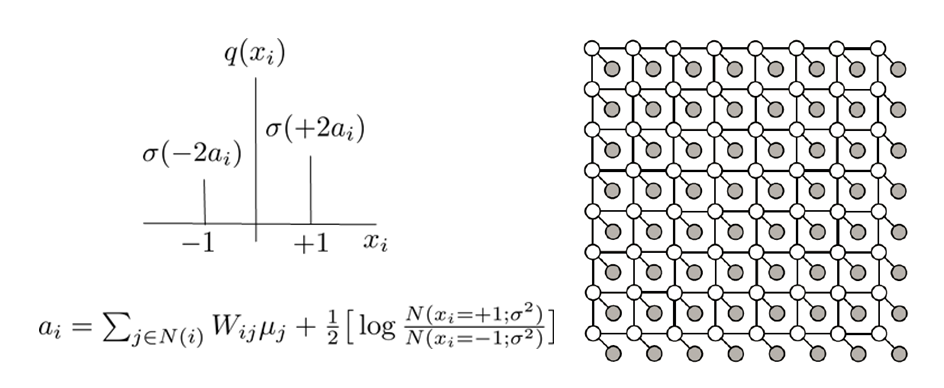
\includegraphics[width=0.8\textwidth, trim={10 10 10 10}]{figures/ising_vi1.png}
    \caption{Mean-field VI approximation (left) and Ising model (right).}
    \label{fig:ising_vi1}
\end{figure}

In order to compute this mean, we need to know the values of $q_j(x_j=+1)$ and $q_j(x_j=-1)$. Let $m_i = \sum_{j\in N(i)}w_{ij}\mu_j$ be the mean value of neighbors and let $L_{i}^{+} = N(x_i=+1,\sigma^2)$ and $L_{i}^{-} = N(x_i=-1, \sigma^2)$, then we can compute the mean as follows:
\begin{eqnarray}
    q_i(x_i=+1) &=& \frac{\exp \{m_i + L_{i}^{+}\}}{\exp \{m_i + L_{i}^{+}\} + \exp \{-m_i + L_{i}^{-}\}} \\
    &=& \frac{1}{1+\exp \{-2m_i + L_{i}^{-} - L_{i}^{+}\}} = \frac{1}{1+\exp \{-2a_i\}} = \sigma(2a_i)
\end{eqnarray}
where $a_i = m_i + 1/2(L_{i}^{+} - L_{i}^{-})$ and $\sigma(x)$ is a sigmoid function. Since $q_i(x_i=-1) = 1-q_i(x_i=+1)=1-\sigma(2a_i)=\sigma(-2a_i)$, we can write the mean of our variational approximation $q_i(x_i)$ as follows:
\begin{equation}
   \mu_i = E_{q_i}[x_i] = \sigma(2a_i) - \sigma(-2a_i) = \tanh(a_i)
\end{equation}
In other words, our mean-field updates of the variational parameters $\mu_i$ at iteration $k$ are computed as follows:
\begin{equation}
    \mu_{i}^{(k)} = \tanh \bigg(\sum_{j\in N(i)}w_{ij}\mu_{j}^{(k-1)} + \frac{1}{2}\bigg[\log \frac{N(x_i=+1,\sigma^2)}{N(x_i=-1,\sigma^2)} \bigg] \bigg)\times \lambda + (1-\lambda)\times \mu_{i}^{(k-1)}
\end{equation}
where we added a learning rate parameter $\lambda \in (0, 1]$. We further note that we can simplify the computation of ELBO term by term as follows:
\begin{eqnarray}
  && \sum_{(s,t)\in E} E_{q(x)}[x_s w_{st} x_t] = \frac{1}{2}\sum_{i=1}^{n}\sum_{j\in N(i)}\bigg(\sum_{x_i \in \{-1,+1\}} \sum_{x_j \in \{-1,+1\}}q_i(x_i)q_j(x_j)x_i J x_j \bigg) = \\
  && \frac{1}{2}\sum_{i=1}^{n}\sum_{j\in N(i)}\bigg(q_i(x_i=+1)JE[x_j] - q_i(x_i=-1)JE[x_j]\bigg) = \frac{1}{2}\sum_{i=1}^{n}\sum_{j \in N(i)} E[x_i] J E[x_j] 
\end{eqnarray}
Similarly,
\begin{eqnarray}
 && E_{q(x)}[\log N(x_i, \sigma^2)] = \sum_{i=1}^{n}\bigg[\sum_{x_i \in \{-1,+1\}}q_i(x_i)\log N(x_i,\sigma^2) \bigg] = \\
 && \sum_{i=1}^{n}\bigg[\sigma(2a_i)\log N(x_i=+1,\sigma^2)+\sigma(-2a_i)\log N(x_i=-1,\sigma^2) \bigg]
\end{eqnarray}

\begin{figure}[hptb]
    \centering
    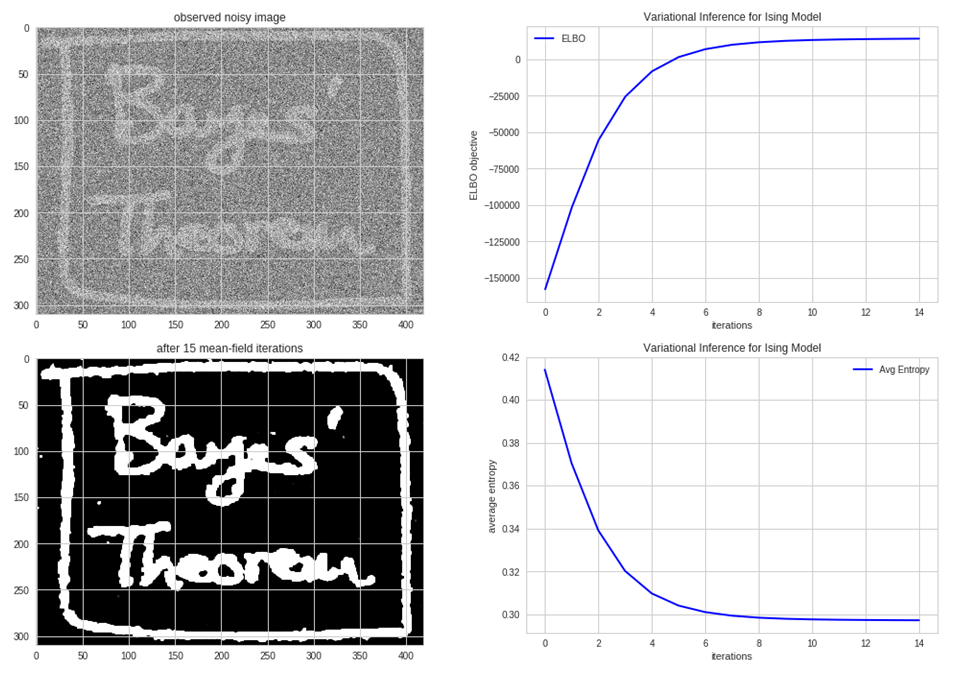
\includegraphics[width=0.8\textwidth, trim={10 10 10 10}]{figures/ising_vi2.png}
    \caption{Image Denoising for Ising model.}
    \label{fig:ising_vi2}
\end{figure}

Figure \ref{fig:ising_vi2} shows experimental results for binary image denoising via mean-field variational inference. The noisy observed image is shown in the top-left obtained by adding Gaussian noise to each pixel and binarizing the image based on mean threshold. We then set the variational inference parameters such as the coupling strength $J=1$, noise level $\sigma = 2$, smoothing rate $\lambda=0.5$ and max number of iterations to $15$. The resulting de-noised binary image is shown in the bottom-left corner of Figure \ref{fig:ising_vi2}. We can also see an increase in the ELBO objective (top-right) and a decrease in the average entropy of our binary random variables $q_i(x_i)$ representing the value of each pixel (bottom-right) as the number of mean-field iterations increases.\\

The 2-D Ising model can be extended in multiple ways, for example: 3-D grids and $K$-states per node (aka Potts model).\\

\subsection{Stochastic Variational Inference}

One limitation of LDA is that the number of topics is fixed ahead of time. A commonly used approach to finding the number of topics $K$ is cross-validation. However, for very large data-sets this approach may not be practical. We can address this issue with a Bayesian non-parametric topic model where the number of topics is learned from data: the Hierarchical Dirichlet Process (HDP) topic model.\\

\begin{figure}[tbhp]
    \centering
    \includegraphics[width=0.25\textwidth, trim={10 10 10 10}]{figures/local_global_gm.png}
    \caption{Graphical model with local and global latent variables.}
    \label{fig:svi_gm}
\end{figure}

While tranditional algorithms require repeatedly analyzing the whole data set before updating the variational parameters, we focus on analyzing randomly sampled subsets. First, we derive the Stochastic Variational Inference (SVI) algorithm for a class of graphical models with global and local laten variables as shown in Figure \ref{fig:svi_gm}. The join distribution factorizes into a product of a global term $\beta$ and local term $z_n$:
\begin{equation}
    p(x,z,\beta|\alpha) = p(\beta|\alpha)\prod_{n=1}^{N}p(x_n,z_n|\beta)
\end{equation}
Our goal is to approximate the posterior distribution of the hidden variables given the observations $p(\beta,z|x)$. We use a variational distribution to approximate the posterior as measured by KL divergence. Variational inference minimizes KL divergence or alternatively maximizes the evidence lower bound (ELBO):
\begin{eqnarray}
    \log p(x) &=& \log \int p(x,z,\beta) dz d\beta \\
              &=& \log \int p(x,z,\beta) \frac{q(z,\beta)}{q(z,\beta)} dz d\beta \\
              &=& \log \bigg(E_q \bigg[\frac{p(x,z,\beta)}{q(z,\beta)} \bigg] \bigg) \\
              &\geq& E_q[\log p(x,z,\beta)] - E_q[\log q(z,\beta)]\\
              &=& L(q)
\end{eqnarray}
The ELBO contains two terms: the first term is the expected log joint $E_q[\log p(x,z,\beta)]$ and the second term is the entropy of the variational distribution $- E_q[\log q(z,\beta)]$. We restrict $q(z,\beta)$ to be in a tractable family of distributions in order to efficiently compute the expectations in the ELBO. We then find the member of the family that maximizes the ELBO and use the optimized distribution as a proxy for the posterior. Solving this maximization problem is equivalent to finding the member of the family that is closest in KL divergence to the posterior:
\begin{eqnarray}
    \min KL(q(z,\beta)||p(z,\beta|x)) &=& E_q[\log q(z,\beta)] - E_q[\log p(z,\beta|x)] \\
    &=& E_q[\log q(z,\beta)] - E_q[\log p(x,z,\beta)] + \log p(x) \\
    &=& -L(q) + \mathrm{const}
\end{eqnarray}
where $\log p(x)$ is replaces by a constant because it does not depend on $q$. The simplest variational family of distributions is the fully factored mean-field family. In this family, each hidden variable is independent and governed by its own parameter:
\begin{equation}
    q(z,\beta) = q(\beta|\lambda)\prod_{n=1}^{N}\prod_{j=1}^{J}q(z_{nj}|\phi_{nj})
\end{equation}
To specify the form of the distribution, we choose $q(\beta|\lambda)$ and $q(z_{nj}|\phi_{nj})$ to be in the exponential distribution with the natural parameters $\lambda$ and $\phi_{nj}$:
\begin{eqnarray}
   q(\beta|\lambda) &=& h(\beta)\exp\{\lambda^{T}t(\beta) - a_{g}(\lambda)\}\\
   q(z_{nj}|\phi_{nj}) &=& h(z_{nj})\exp\{\phi_{nj}^{T}t(z_{nj} - a_{l}(\phi_{nj}))\}
\end{eqnarray}
The mean-field family has several computational advantages. For example the entropy term in the ELBO objective function decomposes:
\begin{equation}
   -E_q[\log q(z,\beta)] = -E_{\lambda}[\log q(\beta)] - \sum_{n=1}^{N}\sum_{j=1}^{J}E_{\phi_{nj}}[\log q(z_{nj})]
\end{equation}
In traditional mean-field variational inference, we maximize $L(q)$ with coordinate ascent: we iteratively optimize each variational parameter while holding the other parameters fixed. Given our assumptions that each conditional is an exponential family, we can optimize each coordinate in closed form. We first derive the coordinate update for the global parameter $\lambda$. Keeping only the terms of $L(q)$ that depend on $\lambda$, we get:
\begin{eqnarray}
    L(\lambda) &=& E_q[\log p(x,z,\beta)] - E_q[\log q(\beta)] + \mathrm{const} \\
    &=& E_q[\log p(\beta|x,z)] - E_q[\log q(\beta)] + \mathrm{const}
\end{eqnarray}
where we used the factorization $p(x,z,\beta) = p(\beta|x,z)p(x,z)$ and absorbed $E_q[p(x,z)]$ into the constant that does not depend on $\lambda$. To derive the coordinate ascent update, we take the gradient \cite{SVI2013}:
\begin{equation}
   \nabla_{\lambda}L = \nabla_{\lambda}^{2}a_g(\lambda)(E_q[\eta_g(x,z,\alpha)] - \lambda) 
\end{equation}
We can set the gradient to zero by setting $\lambda = E_q[\eta_g(x,z,\alpha)]$. This sets the global variational parameter equal to the expected natural parameter of its complete conditional distribution. We now turn to the local parameters $\phi_{nj}$. The gradient is similar to the global case:
\begin{equation}
   \nabla_{\phi_{nj}}L = \nabla_{\phi_{nj}}^{2}a_{l}(\phi_{nj})(E_q[\eta_l(x_n,z_{n,-j},\beta)] - \phi_{nj})
\end{equation}
We can set the gradient to zero by choosing $\phi_{nj} = E_q[\eta_l(x_n,z_{n,-j},\beta)]$. The variational updates form the algorithm for coordinate ascent variational inference, iterating between updates of each local parameter and the global parameter. The full algorithm is described in Algorithm \ref{alg:svi_1} which is guaranteed to find a local optimum of the ELBO.\\

\begin{algorithm}
\caption{Coordinate Ascent SVI \cite{SVI2013}}
\label{alg:svi_1}
\begin{algorithmic}[1]
\STATE Initialize $\lambda^{(0)}$ randomly
\STATE \textbf{repeat}
\STATE ~~~ \textbf{for} each local variational parameter $\phi_{nj}$ \textbf{do}
\STATE ~~~ ~~~ Update $\phi_{nj}^{(t)} = E_{q^{(t-1)}}[\eta_{l,j}(x_n,z_{n,-j},\beta)]$
\STATE ~~~ \textbf{end for}
\STATE ~~~ Update the global variational parameters: $\lambda^{(t)} = E_{q^{(t)}}[\eta_g(z,x)]$
\STATE \textbf{until} the ELBO converges
\end{algorithmic}
\end{algorithm}

We now turn the Hierarchical Dirichlet Process (HDP) topic model. The HDP topic model couples a set of document-level DPs via a single top-level DP \cite{teh2005jasa}. The base distribution $H$ of the top-level DP is a symmetric Dirichlet over the vocabulary simplex. We draw once from this DP: $G_0 \sim DP(\omega, H)$. In the second level, we use $G_0$ as a base measure for a document level DP: $G_d \sim DP(\alpha, G_0)$. As a result, the global topics are shared between documents with different mixing proportions.

\begin{figure}[tbhp]
    \centering
    \includegraphics[width=0.5\textwidth, trim={10 10 10 10}]{figures/hdp_svi_gm.png}
    \caption{HDP graphical model for SVI inference.}
    \label{fig:svi_gm2}
\end{figure}

Figure \ref{fig:svi_gm2} shows a graphical model for the HDP topic model. The generative process of the HDP topic model can be described as follows.
\begin{enumerate}
    \item Draw global topics, $\beta_k \sim \mathrm{Dir}(\eta)$
    \item Draw mixing proportions, $\nu_k \sim \mathrm{Beta}(1,\omega)$
    \item For each document $d$:
    \begin{enumerate}
        \item Draw document-level topic indices, $c_{di} \sim \mathrm{Mult}(\nu)$
        \item Draw document-level mixing proportions, $\pi_{di} \sim \mathrm{Beta}(1,\alpha)$
        \item For each word $n$:
        \begin{enumerate}
            \item Draw topic assignment $z_{dn} \sim \mathrm{Mult}(\pi_d)$
            \item Draw word $w_n \sim \mathrm{Mult}(\beta_{c_{d,z_{dn}}})$
        \end{enumerate}
    \end{enumerate}
\end{enumerate}

In order to implement an infinite number of topics at corpus and document levels we need to truncate our representation to $K$ topics at the corpus level and $T$ topics at the document level. This ways we are optimizing a finite number of variational parameters. We can write down the joint variational family distribution as:
\begin{equation}
    q(\beta,\nu,z,\pi) = \bigg(\prod_{k=1}^{K}q(\beta_k|\lambda_k)q(\nu_k|a_k)\bigg)\bigg(\prod_{d=1}^{D}\prod_{i=1}^{T}q(c_{di}|\zeta_{di})q(\pi_{di}|\gamma_{di})\prod_{n=1}^{N}q(z_{dn}|\phi_{dn}) \bigg)
\end{equation}
The Stochastic Variational Inference (SVI) algorithm is summarized in Algorithm \ref{alg:svi_2}.

\begin{algorithm}
\caption{Stochastic Variational Inference for HDP \cite{SVI2013}}
\label{alg:svi_2}
\begin{algorithmic}[1]
\STATE Initialize $\lambda^{(0)}$ randomly. Set $a^{(0)}=1$ and $b^{(0)}=\omega$
\STATE Set the step-size schedule $\rho_t$
\STATE \textbf{repeat}
\STATE ~~~ Sample a document $w_d$ uniformly from the dataset
\STATE ~~~ For $i \in \{1,...,T\}$, $k \in \{1,...,K\}$: $\zeta_{di}^{k} \propto \exp \{\sum_{n=1}^{N}E[\log \beta_{k,w_{dn}}]\}$
\STATE ~~~ For $n \in \{1,...,N\}$, $i \in \{1,...,T \}$: $\phi_{dn}^{i} \propto \exp\{\sum_{k=1}^{K}\zeta_{di}^{k}E[\log\beta_{k,w_{dn}}]\}$
\STATE ~~~ \textbf{repeat}
\STATE ~~~ ~~~ For $i \in \{1,...,T\}$ set \\
~~~ ~~~ ~~~ ~~~ $\gamma_{di}^{(1)} = 1 + \sum_{n=1}^{N}\phi_{dn}^{i}$\\
~~~ ~~~ ~~~ ~~~ $\gamma_{di}^{(2)} = \alpha + \sum_{n=1}^{N}\sum_{j=i+1}^{T}\phi_{dn}^{j}$\\
~~~ ~~~ ~~~ ~~~ $\zeta_{di}^{k} \propto \exp \{E[\log \sigma_k(V)]+\sum_{n=1}^{N}\phi_{dn}^{i}E[\log \beta_{k,w_{dn}}] \}$, $k \in \{1,...,K\}$
\STATE ~~ ~~~ For $n \in \{1,...,N\}$ set \\
~~~ ~~~ ~~~ ~~~ $\phi_{dn}^{i} \propto \exp \{E[\log \sigma_i(\pi_d)]+\sum_{k=1}^{K}\zeta_{di}^{k}E[\log \beta_{k,w_{dn}}] \}$, $i \in \{1,...,T\}$
\STATE ~~~ \textbf{until} local parameters converge
\STATE ~~~ For $k \in \{1,...,K\}$ set intermediate topics:\\
~~~ ~~~ ~~~ ~~~ $\hat{\lambda}_{kv} = \eta + D\sum_{i=1}^{T}\zeta_{di}^{k}\sum_{n=1}^{N}\phi_{dn}^{i}w_{dn}$\\
~~~ ~~~ ~~~ ~~~ $\hat{a}_k = 1 + D\sum_{i=1}^{T} \zeta_{di}^{k}$\\
~~~ ~~~ ~~~ ~~~ $\hat{b}_k = \omega + D\sum_{i=1}^{T}\sum_{l=k+1}^{K}\zeta_{di}^{l}$
\STATE ~~~ Set \\
~~~ ~~~ ~~~ ~~~ $\lambda^{(t)} = (1-\rho_t)\lambda^{(t-1)} + \rho_t\hat{\lambda}$\\
~~~ ~~~ ~~~ ~~~ $a^{(t)} = (1-\rho_t)a^{(t-1)} + \rho_t\hat{a}$\\
~~~ ~~~ ~~~ ~~~ $b^{(t)} = (1-\rho_t)b^{(t-1)} + \rho_t\hat{b}$
\STATE \textbf{until} end of documents
\end{algorithmic}
\end{algorithm}
where the expectations used in Algorithm \ref{alg:svi_2} are computed as follows:
\begin{eqnarray}
    E[\log \beta_{kv}] &=& \Psi(\lambda_{kv}) - \Psi(\sum_{v^{\prime}}\lambda_{kv^{\prime}})\\
    E[\log \sigma_k(V)] &=& \Psi(a_k) - \Psi(a_k+b_k) + \sum_{l=1}^{k-1}[\Psi(b_l)-\Psi(a_l+b_l)]
\end{eqnarray}

The on-line variational inference algorithm for Hierarchical Dirichlet Process was used to fit a topic model on the 20newsgroups dataset. The dataset consists of $11,314$ documents and over $100K$ unique tokens. Standard text pre-processing was used including tokenization, stop-word removal and stemming. A compressed dictionary of $4K$ words was constructed by filtering out tokens that appear in less than $5$ documents and more than $50\%$ of the corpus. The top-level truncation was set to $T=20$ topics and the second level truncation was set to $K=8$ topics. The concentration parameters were chosen as $\gamma = 1.0$ at the top-level and $\alpha=0.1$ at the group level to yield a broad range of shared topics that are concentrated at the group level. Figure \ref{fig:hdp_topics_vb} shows a sample of the global level topics inferred by online variational HDP algorithm. We can find topics about autos, politics and for sale items that correspond to the target labels of the 20newsgroups dataset.

\begin{figure}[thpb]
    \centering
    \includegraphics[width=0.8\textwidth, trim={10 10 10 10}]{figures/hdp_topics.png}
    \caption{Sample of HDP topics inferred using online variational bayes algorithm on 20newsgroups dataset.}
    \label{fig:hdp_topics_vb}
\end{figure}

\subsection{Normalizing Flows}

A normalizing flow describes the transformation of a probability density through a sequence of invertible mappings \cite{Rezende2015}. The target density is approximated through a flow of the prior distribution through a sequence of invertible (one-to-one) transformations resulting in the target posterior density.\\

The basic rule for transformation of densities considers an invertible, smooth mapping $f: \mathbb{R}^{d}\rightarrow \mathbb{R}^{d}$. Recall, that in the case of discrete random variables, for a one-to-one $y=f(x)$ where $X \sim p(x)$, the transformed density is $p_y(y) = \sum_{\{x : y = f(x)\}} p_x(x)$. If $X$ is a continuous random variable, we can differentiate the CDF to obtain an expression for the transformed density:
\begin{eqnarray}
   F_{y}(y) &=& P(Y \leq y) = P(f(X) \leq y) = P(X \leq f^{-1}(y)) \\
   p_{y}(y) &=& \frac{d}{dy}F_{y}(y) = \frac{d}{dy}P(X \leq f^{-1}(y)) = \frac{dx}{dy}\frac{d}{dx}P(X \leq f^{-1}(y)) = p_x(x)|\frac{dx}{dy}|
\end{eqnarray}
The above expression generalizes for high dimensional transformations using a Jacobian:
\begin{equation}
    p_y(y) = p_x(x)|\mathrm{det}\bigg(\frac{\partial x}{\partial y}\bigg)|
\end{equation}
Let's examine a $k$ step transformation:
\begin{equation}
    z_k = f_k \circ f_{k-1} \circ \cdots \circ f_{2} \circ f_{1} (z_0) = f_k(f_{k-1}(\cdots f_{2}(f_{1}(z_0))))
\end{equation}
For $k=1$, we have $z_1 = f_{1}(z_0)$, where $z_0 \sim q_{0}(z_0)$ and
\begin{equation}
   q_{1}(z_1) = q_{0}(z_0)|\mathrm{det}\bigg(\frac{\partial z_0}{\partial z_1}\bigg)|  = q_{0}(z_0)|\mathrm{det}\bigg(\frac{\partial f_{1}^{-1}}{\partial z_1}\bigg)| = q_{0}(z_0)|\mathrm{det}\bigg(\frac{\partial f_{1}}{\partial z_0}\bigg)|^{-1}  
\end{equation}
For $k=2$, we have $z_2 = f_2 \circ f_1 (z_0) = f_2(f_1(z_0)) = f_2(z_1)$ that we can re-write as:
\begin{equation}
    q_{2}(z_2) = q_1(z_1)|\mathrm{det}\bigg(\frac{\partial f_2}{\partial z_1} \bigg)|^{-1} =  q_{0}(z_0)|\mathrm{det}\bigg(\frac{\partial f_{1}}{\partial z_0}\bigg)|^{-1} \times |\mathrm{det}\bigg(\frac{\partial f_2}{\partial z_1} \bigg)|^{-1} 
\end{equation}
Generalizing for $k$ steps, we have:
\begin{equation}
    q_{k}(z_k) = q_{0}(z_0)|\mathrm{det}\bigg(\frac{\partial f_{1}}{\partial z_0}\bigg)|^{-1} \times |\mathrm{det}\bigg(\frac{\partial f_2}{\partial z_1} \bigg)|^{-1} \times \cdots \times |\mathrm{det}\bigg(\frac{\partial f_k}{\partial z_{k-1}}\bigg)|^{-1} 
\end{equation}
Taking the log, we can represent this compactly as:
\begin{equation}
    \log q(z_k) = \log q(z_0) - \sum_{i=1}^{K}\log|\mathrm{det}\bigg(\frac{\partial f_i}{\partial z_{i-1}}\bigg)|
\end{equation}






\newpage
\section{Optimization}
\subsection{Natural Gradient Descent}

Let's define the score function $s(\theta) = \nabla_{\theta}\log p(x|\theta)$, the Fisher information matrix is given by $I(\theta) = -E\bigg[\nabla_{\theta}^{2}\log p(x|\theta) \bigg]$ or in the matrix form:
\begin{equation}
    \bigg[I(\theta)\bigg]_{ij} = -E \bigg[\frac{\partial^2}{\partial \theta_i \partial \theta_j}\log p(x|\theta) \bigg]
\end{equation}
The second order Taylor expansion of KL divergence is
\begin{equation}
    KL(p_{\theta}||p_{\theta+d}) = KL(p_{\theta}||p_{\theta}) - E_{p(x|\theta)}[\nabla_{\theta}\log p(x|\theta)]^{T}d + \frac{1}{2}d^{T}I(\theta)d \approx \frac{1}{2}d^{T}I(\theta)d 
\end{equation}
We would like to find a vector $d$ that minimizes the loss function $L(\theta)$:
\begin{equation}
    d^{\ast} = \arg \min_{d s.t. KL(p_{\theta}||p_{\theta+d}) = c} L(\theta + d)
\end{equation}
We can re-write the above constrained problem as a Lagrangian:
\begin{eqnarray}
    d^{\ast} &=& \arg \min_d L(\theta + d) + \lambda (KL(p_{\theta}||p_{\theta + d})-c) \\
    &\approx& \arg \min L(\theta) + \nabla_{\theta}L(\theta)^{T}d + \frac{1}{2}d^{T}I(\theta)d - \lambda c
\end{eqnarray}
Setting the derivative wrt to $d$ to zero, we get:
\begin{eqnarray}
    0 &=& \nabla_{\theta}L(\theta) + \lambda I(\theta) d \\
    d &=& -\frac{1}{\lambda}I(\theta)^{-1}\nabla_{\theta}L(\theta)
\end{eqnarray}
Thus, our optimal $d$ is in the opposite direction of the gradient preconditioned by inverse of Fisher information matrix. The natural gradient is defined as
\begin{equation}
    \tilde{\nabla}_\theta L (\theta) = I(\theta)^{-1}\nabla_{\theta}L(\theta)
\end{equation}

\subsection{Non-Convex Optimization}

Non-convex problems are NP hard to solve and in general no algorithmic technique is expected to succeed at finding global optima solutions to these problems. However, non-convex problems that have a certain structure can be solved in polynomial time, such as projections on non-convex constraints and structural properties of the objective funcions (e.g. marginal convexity) \cite{NonConvexML}

\subsubsection{Projected Gradient Descent}

Exploiting the projected gradient descent algorithm with non-convex problems requires projections onto non-convex sets:
\begin{equation}
    \Pi_{C}(z) = \arg \min_{x \in C} ||x-z||_2
\end{equation}
The projection problem above can itself be NP hard. However, for several well-structured sets, projections can be carried out efficiently despite the sets being non-convex. For example, projecting into sparse vectors:
\begin{equation}
    \hat{w} = \arg \min_{||w||_0 \leq s} \sum_{i=1}^{n}\big(y_i - x_{i}^{T}w \big)^{2}
\end{equation}
The projection above can be done by sorting co-ordinates of the $z$ vector in descending order and setting all except that top $s$ coordinates to zero. Similarly, projections into low-rank matrices as used in recommendation systems:
\begin{equation}
    \hat{A_{lr}} = \arg \min_{rank(X) \leq r}\sum_{(i,j)\in \Omega}\big(X_{ij} - A_{ij}\big)^{2}
\end{equation}
The projection above can be done by applying singular value decomposition of the matrix $A$ and keeping the top $r$ singular values and vectors. Non-convex projections are used in the generalized Projected Gradient Descent (PGD) summarized in Algorithm \ref{alg:general_pgd}.

\begin{algorithm}
\caption{Generalized Projected Gradient Descent}
\label{alg:general_pgd}
\begin{algorithmic}[1]
\STATE \textbf{Input:} objective function $f$, constraint set $C$, step length $\eta$
\STATE \textbf{Output:} A point $\hat{x} \in C$ with near-optimal objective value
\STATE $x^{1} \leftarrow 0$
\STATE \textbf{for} t = 1,2,...,T \textbf{do}
\STATE ~~~ $z^{t+1} = x^{t} - \eta \nabla f(x^{t})$
\STATE ~~~ $x^{t+1} = \arg \min_{x \in C}||x - z^{t+1}||$
\STATE \textbf{end for}
\STATE option 1: \textbf{return} $\hat{x}_{final} = x^{T}$
\STATE option 2: \textbf{return} $\hat{x}_{avg} = \frac{1}{T}\sum_t x^{t}$
\STATE option 3: \textbf{return} $\hat{x}_{best} = \arg \min_{t \in [T]} f(x^{t})$
\end{algorithmic}
\end{algorithm}
We can see two alternating steps of moving in the direction opposite to the gradient and projecting the resulting vector on our non-convex constrain set. 

\subsubsection{Alternating Minimization}

Alternating Minimization (AM) is a widely used non-convex optimization technique. The popular K-means clustering algorithm and the EM algorithm for latent variable models are problem-specific variants of the general alternating minimization principle. The alternating minimization principle is most often used in settings where the optimization problem consists of two or more groups of variables. For example, in a collaborative filtering recommendation system, the objective function is not jointly convex, however, it is \textit{marginally convex}:
\begin{equation}
    \hat{A}_{lv} = \arg \min_{U \in R^{m\times r}, V \in R^{n\times r}} \sum_{(i,j)\in \Omega}\big(U_{i}^{T}V_{j} - A_{i,j}\big)^{2}
\end{equation}
For a group of two variables, we can write down alternative minimization as in Algorithm \ref{alg:alt_min}
\begin{algorithm}
\caption{Alternating Minimization}
\label{alg:alt_min}
\begin{algorithmic}[1]
\STATE \textbf{Input:} objective function $f: X \times Y \rightarrow R$
\STATE \textbf{Output:} A point $\hat{x} \in X \times Y$ with near-optimal objective value
\STATE $(x^{1}, y^{1}) \leftarrow \mathrm{INIT}()$
\STATE \textbf{for} t = 1,2,...,T \textbf{do}
\STATE ~~~ $x^{t+1} = \arg \min_{x \in X} f(x, y^t)$
\STATE ~~~ $y^{t+1} = \arg \min_{y \in Y} f(x^{t+1}, y)$
\STATE \textbf{end for}
\STATE \textbf{return} $(x^{T}, y^{T})$
\end{algorithmic}
\end{algorithm}

The idea of solving several intermediate marginal optimization problems instead of a single big optimization problem is the key to practical success of alternating minimization algorithm. Algorithms similar to alternating minimization are commonly known as Coordinate Descent (CD) and are very popular for large scale convex optimization problems. The coordinate descent treats a single $p$ dimensional variable $x \in R^{p}$ as $p$ one-dimensional variables $\{x_1,...,x_p\}$ and executes AM like steps resulting in intermediate problems being uni-dimensional. A variant of Coordinate Descent splits variables into blocks of multi-dimensional variables and minimizes over one block of variables at each time step. 

\subsubsection{Stochastic Optimization Techniques}

One of the main hurdles in achieving local optimality in high dimensional problems are saddle points. Saddle points are characterized by zero gradient and Hessian matrix with both positive and negative eigen values. They stall the progress of optimization methods such as gradient descent due to the vanishing gradient while not characterizing the function in any useful way in contrast to local optima. However, saddle points are unstable and a slight perturbation is likely to cause gradient descent to roll down the function surface. This motivates stochastic optimization techniques.

Saddle points can often be caused by symmetry of the objective function and they increase exponentially with the dimension of the problem. This motivates the application of Noisy Gradient Descent (NGD) Algorithm \ref{alg:noisy_gd}.

\begin{algorithm}
\caption{Noisy Gradient Descent}
\label{alg:noisy_gd}
\begin{algorithmic}[1]
\STATE \textbf{Input:} objective $f$, constraint set $C$, max step length $\eta_{\max}$, tolerance $\epsilon$
\STATE \textbf{Output:} A locally optimal point $\hat{x} \in R^{p}$ 
\STATE $x^{1} \leftarrow \mathrm{INIT}()$
\STATE Set $T = 1/\eta^{2}$, where $\eta = \min\{\epsilon^{2}/\log^{2}(1/\epsilon),\eta_{\max}\}$
\STATE \textbf{for} t = 1,2,...,T \textbf{do}
\STATE ~~~ sample perturbation $\zeta^{t} \sim S^{p-1}$ //random point on a unit sphere
\STATE ~~~ $g^{t} = \nabla f(x^{t}) + \zeta^{t}$
\STATE ~~~ $x^{t+1} = \Pi_{C}(x^{t} - \eta g^{t})$ //project onto constraint set
\STATE \textbf{end for}
\STATE \textbf{return} $x^{T}$
\end{algorithmic}
\end{algorithm}

The technique of using randomly pertrubed (stochastic) gradients to escape saddle ponts is part of a more general framework of Langevin Dynamics which studies the case when the perturbations are not isotropic or are applied at a scale that adapts to the problem. 

\subsubsection{Simulated Annealing}

Simulated Annealing (SA) is a stochastic algorithm that attempts to find the global optimum of an objective function $f(x)$. The method is inspired by statistical physics, in particular the Boltzmann distribution that specifies the probability of being in a particular state $x$:
\begin{equation}
    p(x) \propto \exp\{-f(x)/T\}
\end{equation}
where $f(x)$ is the energy of the system and $T$ is the temperature. As the temperature approaches zero, the system spends more and more time in its minimum energy (most probable) state. As the temperature decreases, the largest peaks become larger and the smallest peaks dissappear. By cooling slowly enough, it is possible to track the largest peak and therefore find the global optimum.\\

Simulated annealing is closely related to the Metropolis-Hastings algorithm for generating samples from a probability distribution. At each step of the algorithm, we sample a new state according to a proposal distribution $x^{\prime} \sim q(\dot|x_k)$, such as a random walk proposal:
\begin{equation}
    x^{\prime} = x_k + \epsilon_k, ~~~ \mathrm{where}~ \epsilon_k \sim N(0,\Sigma)
\end{equation}
Having proposed a new state, we compute $\alpha$ as in Algorithm \ref{alg:sim_annealing}.
\begin{algorithm}
\caption{Simulated Annealing}
\label{alg:sim_annealing}
\begin{algorithmic}[1]
\STATE $\alpha = \exp\{(f(x)-f(x^{\prime}))/T\}$
\STATE $r = \min(1,\alpha)$
\STATE $u \sim \mathrm{Unif}(0,1)$
\STATE if $u < r$ 
\STATE ~~~ $x_{k+1} = x^{\prime}$
\STATE else
\STATE ~~~ $x_{k+1} = x_k$
\STATE end if  
\end{algorithmic}
\end{algorithm}
Thus, if a new state has lower energy (higher probability), we will definitely accept it but if it has higher energy (lower probability), we might still accept it depending on the temperature. Therefore, the algorithm allows downhill moves in probability space but less frequently as the temperature drops. In practice it is common to use an exponential cooling schedule: $T_k = T_0 C^{k}$, where $T_0 \sim 1$ is the initial temperature and $C \sim 0.8$ is the cooling rate. Cooling too quickly can result in getting stuck in local optima, while cooling too slowly wastes time. The optimum cooling schedule is difficult to determine.    

\begin{figure}[tbhp]
    \centering
    \includegraphics[width=0.9\textwidth, trim={10 10 10 10}]{figures/sim_annealing_merged.png}
    \caption{Simulated Annealing}
    \label{fig:sim_annealing_merged}
\end{figure}

Figure \ref{fig:sim_annealing_merged} shows the objective $f(x)$ at two different temperatures (left). The function appears more peaky when the temperature is lower. We can also see that the method stochastically reduces the energy over time for the given cooling schedule (middle). Finally a histogram of samples shows that most samples are concentrated near the global maximum (right).


\subsection{Bayesian Optimization}

Machine learning algorithms frequenty require careful tuning of hyperparameters. Often exhaustive and computationally expensive methods such as grid search cross validation are used to find model parameters that optimize a suitable performance objective. An alternative to grid search is randomized parameter optimization that samples parameter settings from a distribution over possible parameter values. This has two main benefits over the exhaustive search: the number of iterations can be chosen independent of the number of parameters and adding parameters that do not influence performance does not decrease efficiency. Rather than exploring the parameter space randomly (according to a chosen distribution), it would be great to adapt an active learning approach that selects parameter values in a way that reduces uncertainty and provides a balance between exploration and exploitation. Bayesian optimization provides an automated Bayesian framework by utilizing Gaussian Processes (GPs) to model algorithm's generalization performance \cite{snoek2012}.\\

Bayesian optimization assumes that a suitable performance function was sampled from a Gaussian Process and maintains a posterior distribution for this function as observations are made: $f(x)\sim \mathrm{GP}(m(x),\kappa(x,x^{\prime}))$. To choose which hyperparameters to explore next, one can optimize the Expected Improvement (EI) over the current best result or the Gaussian process Upper Confidence Bound (UCB). EI and UCB have been shown to be efficient in the number of function evaluations required to find the global optimum of multi-modal black-box functions. Bayesian optimization uses all of the information available from previous evaluations of the objective function as opposed to relying on local gradient and Hessian approximations. This results in an automated procedure that can find an optimum of non-convex functions with relatively few evaluations, at the cost of performing more computation to determine the next point to try. This is particularly useful when evaluations are expensive to perform such as in selecting hyperparameters for deep neural networks.\\

To determine what point should be evaluated next, we need to choose and acquisition function which is used to construct a utility function from the GP posterior. In general, the acquisition function depends on previous observations as well as GP hyperparameters that we denote as $a(x;\{x_n,y_n\},\theta)$, then $x_{next} = \arg \max_x a(x)$. Let $\mu(x;\{x_n,y_n\},\theta)$ be the predictive GP mean function, $\sigma^{2}(x;\{x_n,y_n\},\theta)$ be the predictive GP variance function and $\Phi(x)$ be the cumulative distribution function of the standard normal. Then we can define the following acquisition functions.\\

\textit{Probability of Improvement}. This strategy maximizes the probability of improving over the best current value. This can be computed as follows:
\begin{equation}
    a_{PI}(x;\{x_n,y_n\},\theta) = \Phi(\gamma(x)), ~~~~ \gamma(x) = \frac{f(x_{best}) - \mu(x; \{x_n,y_n\},\theta)}{\sigma(x;\{x_n,y_n\},\theta)}
\end{equation}

\textit{Expected Improvement}. Alternatively, one could choose to maximize the expected improvement (EI) over the current best. 
\begin{equation}
    a_{EI}(x;\{x_n,y_n\},\theta) = \sigma(x;\{x_n,y_n\},\theta)(\gamma(x)\Phi(\gamma(x))+N(\gamma(x);0,1))
\end{equation}

\textit{Upper Confidence Bound}. UCB is the idea of exploiting upper confidence bounds to construct acquisition functions that minimize regret over the course of their optimization. These acquisition functions have the following form:
\begin{equation}
    a_{UCB}(x;\{x_n,y_n\},\theta) = \mu(x;\{x_n,y_n\},\theta) - \kappa \sigma(x;\{x_n,y_n\},\theta)
\end{equation}
where $\kappa$ is a tunable acquisition parameter to balance exploration and exploitation. The optima of acquisition functions are located where the uncertainty in GP posterior is large (exploration) and/or where the GP prediction is high (exploitation). Since acquisition functions have analytical forms that are simple to evaluate, they are easier to optimize then the original objective function.\\

An important practical consideration for Bayesian optimization is an appropriate choice of GP kernel and its associated hyperparameters. Squared exponential kernel is often a default choice for Gaussian process regression. However, sample functions with this kernel are too smooth for practical optimization problems. Instead the following ARD Matern $5/2$ kernel is proposed:
\begin{eqnarray}
    K_{M52}(x,x^{\prime}) &=& \theta_0\bigg(1+\sqrt{5r^2(x,x^{\prime})}+\frac{5}{3}r^2(x,x^{\prime}) \bigg)\exp \{-\sqrt{5r^2(x,x^{\prime})}\}\\
    r^2(x,x^{\prime}) &=& \sum_{d=1}^{D}(x_d - x^{\prime}_d)^{2}/\theta_{d}^{2}
\end{eqnarray}
This kernel results in sample functions that are twice-differentiable without requiring the smoothness of the squared exponential kernel. The associated kernel hyperparameters are $D$ length scales $\theta_{1:D}$, the covariance amplitude $\theta_0$, the observation noise $\nu$ and a constant mean $m$. An additional assumption made by GP regression is that the underlying process is stationary, i.e. we can re-write the kernel $k(x,x^{\prime})$ as a function of $x-x^{\prime}$. Intuitively, a function whose length scale does not change throughout the input space will be modelled well by a GP with a stationary kernel.\\ 

Bayesian Optimization algorithm is summarized in Algorithm \ref{alg:bayes_opt}.
\begin{algorithm}
\caption{Bayesian Optimization}
\label{alg:bayes_opt}
\begin{algorithmic}[1]
\STATE \textbf{for} $n=1,2,...$ \textbf{do}
\STATE ~~~ select new $x_{n+1}$ by optimizing acquisition function $\alpha$\\
~~~ ~~~ $x_{n+1} = \arg \max_x \alpha(x;D_n,\theta)$
\STATE ~~~ query objective function to obtain $y_{n+1} = f(x_{n+1})$
\STATE ~~~ augment data $D_{n+1} = \{D_n,(x_{n+1},y_{n+1})\}$
\STATE ~~~ update GP posterior and acquisition function 
\STATE \textbf{end for}  
\end{algorithmic}
\end{algorithm}


\begin{figure}[tbhp]
    \centering
    \includegraphics[width=0.95\textwidth, trim={10 10 10 10}]{figures/bayes_opt.png}
    \caption{Bayesian Optimization of SVM and Random Forest parameters}
    \label{fig:bayes_opt}
\end{figure}

Figure \ref{fig:bayes_opt} shows Baeysian optimization applied to SVM and Random Forest. F1 score was used as performance objective function for a classification task. The figure on the left shows Bayesian optimization of F1 score as a function of the gamma parameter of the SVM RBF kernel: $K(x,x^{\prime}) = \exp\{-\gamma ||x-x^{\prime}||^{2}\}$. We can see that after only 7 iterations we have discovered the gamma parameter that gives the maximum F1 score. The peak of EI utility function at the bottom tells us which experiment to perform next. The figure on the right shows Bayesian optimization of F1 score as a function of maximum depth and the number of estimators of a Random Forest classifier. From the heatmap, we can tell that the maximum F1 score is achieved for $158$ estimators with depth equal to $10$.    


\subsection{Active Learning}

The key idea behind active learning is that a machine learning algorithm can achieve greater accuracy with fewer training labels if it is allowed to choose the data from which it learns. Active learning is well motivated in many modern machine learning problems where unlabeled data may be abundant but labels are expensive to obtain. Active learning is sometimes called query learning or optimal experimental design because an active learner poses queries in the form of unlabelled data instances to be labeled by an oracle. In this way, the active learner seeks to achieve high accuracy using as few labeled instances as possible \cite{Settles2009}.\\

We focus on \textit{pool-based sampling} that assumes that there is a small set of labeled data $L$ and a large pool of unlabelled data $U$. Queries are selectively drawn from the pool according to an informativeness measure. Pool based methods rank the entire collection of unlabelled data to select the best query. Therefore, for very larget data-sets, stream-based sampling maybe more appropriate where the data is scanned sequentially and query decisions are evaluated individually.\\

\begin{figure}[tbhp]
    \centering
    \includegraphics[width=0.95\textwidth, trim={10 10 10 10}]{figures/active_learning_logreg.png}
    \caption{Random Subsampling vs Uncertainty Sampling}
    \label{fig:al_logreg}
\end{figure}

Figure \ref{fig:al_logreg} shows an example of pool-based active learning based on binary classification of a synthetic dataset with two balanced classes using Logistic Regression (LR). On the left, we can see the LR decision boundary as a result of training on a randomly subsampled set of $30$ labels that achieves a classification accuracy of $90\%$ on held out data. On the right, we can see the LR decision boundary as a result of training on $30$ queries selected by uncertainty sampling based on entropy. Uncertainty sampling achieves a higher classification accuracy of $92.5\%$ on the held out set.   


\subsubsection{Query Strategies}

\textit{Uncertainty Sampling.} One of the simplest and most commonly used query framework is uncertainty sampling. In this framework, an active learner queries the label about which it is least certain. For example, in binary logistic regression, uncertainty sampling queries points near the boundary where the probability of being positive is close to $0.5$. For multi-class problems, uncertainty sampling can query points that are least confident:
\begin{equation}
    x_{LC}^{\ast} = \arg \max_x 1 - P_{\theta}(\hat{y}|x)
\end{equation}
where $\hat{y} \in \{1,...,K\}$ is the class label with the highest posterior probability under the model $\theta$. The criterion for the least confident strategy only considers information about the most probable label. We can use max margin sampling to preserve information about the remaining label distribution:
\begin{equation}
    x_{M}^{\ast} = \arg \min_x P_{\theta}(\hat{y}_1|x) - P_{\theta}(\hat{y}_2|x)
\end{equation}
where $\hat{y}_1$ and $\hat{y}_2$ are the first and second most probable class labels under the model, respectively. Intuitively, instances with large margins are easy to classify. Thus, points with small margins are ambiguous and knowing their labels would help the model to more effectively discriminate between them. However, for multi-class problems with very large label sets, the margin strategy still ignores much of the output distribution for the remaining classes. A more general uncertainty sampling strategy is based on entropy:
\begin{equation}
    x_{H}^{\ast} = \arg \max_x -\sum_i P_{\theta}(y_i|x)\log P_{\theta}(y_i|x)
\end{equation}
By learning labels that have highest entropy we can reduce label uncertainty. Uncertainty sampling also works for regression problems, in which case the learner queries the point with highest output variance in its prediction.\\

\textit{Query by Committee.} Another query selection framework is the Query By Committee (QBC) algorithm that involves maintaining a committee $C = \{\theta^{(1)},...,\theta^{(C)}\}$ of models which are all trained on the current labeled set $L$ but represent competing hypotheses. Each committee member is then allowed to vote on the labelings of query candidates and the most informative query is considered to be an instance about which they most disagree. The objective of QBC is to minimize a set of hypotheses that are consistent with the current labeled training data $L$. For measuring the level of disagreement two main approaches have been proposed \cite{Settles2009}: the vote entropy and KL divergence. The vote entropy is defined as follows:
\begin{equation}
    x_{VE}^{\ast} = \arg \max_x - \sum_i \frac{V(y_i)}{C} \log \frac{V(y_i)}{C}
\end{equation}
where $y_i \in \{1,...,K\}$ is the class label, $V(y_i)$ is the number of votes that a label received from the committee members and $C$ is the size of the committee. The KL divergence for QBC voting is defined as follows:
\begin{eqnarray}
    x_{KL}^{\ast} &=& \arg \max_x \frac{1}{C} \sum_{c=1}^{C} KL(P_{\theta^{(c)}}||P_C)\\
    KL(P_{\theta^{(c)}}||P_C) &=& \sum_i P_{\theta^{(c)}}(y_i|x) \log \frac{P_{\theta^{(c)}}(y_i|x)}{P_C(y_i|x)}\\
    P_C(y_i|x) &=& \frac{1}{C}\sum_{c=1}^{C}P_{\theta^{(c)}}(y_i|x)
\end{eqnarray}
where $\theta^{(c)}$ represents a member model of the committee and $P_C(y_i|x)$ is the consensus probability that $y_i$ is the correct label. The KL divergence metric considers the most informative query to be the one with the largest average difference between the label distributions of any one committee member and the consensus distribution.\\

\textit{Variance Reduction}. We can reduce the generalization error by minimizing output variance. Consider a regression problem for which the learning objective is to minimize the mean squared error. Let $\bar{\theta} = E[\hat{\theta}]$ be the expected value of the parameter estimate $\hat{\theta}$ and let $\theta^{\ast}$ be the ground truth, then
\begin{eqnarray}
   \mathrm{MSE} &=& E\bigg[(\hat{\theta} - \theta^{\ast})^{2} \bigg]  = E\bigg[\big[(\hat{\theta} - \bar{\theta})+(\bar{\theta} - \theta^{\ast}) \big]^{2} \bigg] \\
                &=& E\bigg[(\hat{\theta} - \bar{\theta})^{2} \bigg] + 2(\bar{\theta}-\theta^{\ast})E\bigg[\hat{\theta}-\bar{\theta}\bigg] + (\bar{\theta}-\theta^{\ast})^{2} \\
                &=& E\bigg[(\hat{\theta} - \bar{\theta})^{2} \bigg] +  (\bar{\theta}-\theta^{\ast})^{2} \\
                &=& \mathrm{VAR}[\hat{\theta}] + \mathrm{bias}^{2}(\hat{\theta})
\end{eqnarray}
This is called the \textbf{bias-variance tradeoff}. Thus, it is possible to achieve lower MSE with a biased estimator as long as it reduces the variance. A natural question is how low can the variance be? The answer is given by the Cramer-Rao lower bound that provides a lower bound on the variance of any unbiased estimator.
\begin{theorem}
(Cramer-Rao Lower Bound) Assuming $p(x|\theta)$ satisfies the regularity condition, the variance of any unbiased estimator $\hat{\theta}$ satisfies:
\begin{equation}
    \mathrm{VAR}(\hat{\theta}) \geq \frac{1}{-E\big[\frac{\partial^{2} \log p(x|\theta)}{\partial \theta^{2}} \big]} = \frac{1}{I(\theta)}
\end{equation}
where $I(\theta)$ is the Fisher information matrix. 
\end{theorem}
Thus, the Minimum Variance Unbiased (MVU) estimator achieves the minimum variance equal to the inverse of the Fisher information matrix. To minimize variance of parameter estimates, an active learner should select data that maximizes its Fisher information. For multi-variate models with $K$ parameters, Fisher information takes the form of a $K\times K$ matrix:
\begin{equation}
    [I(\theta)]_{ij} = -E \bigg[\frac{\partial^{2}\log p(x|\theta)}{\partial \theta_i \partial \theta_j} \bigg]
\end{equation}
As a result, there are several options for minimizing the inverse information matrix: A-optimality minimizes the trace: $Tr(I^{-1}(\theta))$, D-optimality minimizes the determinant: $|I^{-1}(\theta)|$ and E-optimality minimizes the maximum eigenvalue: $\lambda_{max}[I^{-1}(\theta)]$.\\

However, there are some computational disadvantages to the variance reduction methods. Estimating output variance requires inverting a $K\times K$ matrix for each unlabeled instance, resulting in a time complexity of $\mathcal{O}(UK^{3})$, where $U$ is the size of the query pool. As a result variance reduction methods are empirically slower than simpler query strategies like uncertainty sampling.\\  

Active learning and \textit{semi-supervised learning} both try to make the most of unlabeled data. For example, a basic semi-supervised technique is self-training in which the learner is first trained with a small amount of labeled data and then used to classify the unlabeled data. The most confident unlabeled instances together with their predicted labels are added to the training set and the process repeats.\\ 

\begin{figure}[tbhp]
    \centering
    \includegraphics[width=0.95\textwidth, trim={10 10 10 10}]{figures/active_learning_merged.png}
    \caption{Active Learning: Uncertainty Sampling and Query By Committee.}
    \label{fig:al_merged}
\end{figure}

Figure \ref{fig:al_merged} compares $3$ uncertainty sampling techniques: least confident, max margin and entropy with a random subsampling baseline on 20 newsgroups dataset classified with Logistic Regression. All three methods achieve higher accuracy in comparison to baseline that highlights the benefit of active learning. On the right, we can see the performance of Query By Committee strategy applied to MNIST dataset. The committee consists of $5$ instances of Logistic Regression. Two methods are compared against the random subsampling baseline: vote entropy and average KL divergence. We can see that average KL divergence achieves highest classification accuracy. All experiments were repeated $10$ times.  


\subsection{Submodular Optimization}

Many observation selection problems satisfy an intuitive \textbf{diminishing returns} property: adding an observation helps more if we made few observations so far, and helps less if we already made a lot of observations. From a sensing perspective, combining two sets of information has less gain than the sum of information gains of the individual sets. This concept is formalized by the property of submodularity.\\

Submodularity is a property of \textit{set functions} $f: 2^{V} \rightarrow \mathbb{R}$ that assign each subset $S \subseteq V$ a value $f(S)$. $F$ is called \textit{submodular} if for all $A, B \subseteq V$ it holds that
\begin{equation}
    F(A) + F(B) \geq F(A \cup B) - F(A \cap B)
\end{equation}
Note that if $F$ is non-negative ($F(A)\geq 0$ for all $A$) submodularity implies subadditivity: $f(A \cup B) \leq f(A) + f(B)$. An alternative definition of submodular functions is the following. A set function is sub-modular iff for all $A \subseteq B \subseteq V$ and $s \in V \setminus B$, it holds that
\begin{equation}
    F(A \cup \{s\}) - F(A) \geq F(B \cup \{s\}) - F(B) 
\end{equation}
We can usually check more easily for monotonicity and submodularity of a function via its incremental definition, where the increment function $f(A|B)$ is defined as $f(A|B) = f(A \cup B) - f(B)$. Thus, for a single element $\{e\} \in V \setminus B$ and $A \subseteq B \subseteq V$, we can define sub-modularity as:
\begin{equation}
    f(e|A) \geq f(e|B)
\end{equation}
An important subclass of submodular functions are those which are \textit{monotone} where enlarging the argument set cannot cause the function to decrease. A function $f: 2^{V}\rightarrow \mathbb{R}$ is monotone if for every $A \subseteq B \subseteq V$, we have $f(A) \leq f(B)$.

Submodularity is closed under the operations of non-negative addition, restriction and conditioning. 
\begin{theorem}
(Submodularity is closed under conic combination). Given submodular functions $f_1,f_2,...,f_n$ and $\alpha_i \geq 0$, their conic combination (non-negative addition) is submodular.
\begin{equation}
    f(A) = \sum_{i=1}^{n} \alpha_i f_i(A)
\end{equation}
\end{theorem}
\textit{Proof}. Since every function $f_i$ is submodular and $\alpha_i \geq 0$, we have for $A \subseteq B$:
\begin{equation}
    f_i(j|A) \geq f_i(j|B) \Rightarrow \sum_{i=1}^{n}\alpha_i f_i(j|A)\geq \sum_{i=1}^{n}\alpha_i f_i(j|B) \Rightarrow f(j|A) \geq f(j|B)
\end{equation}

\begin{theorem}
(Entropy is submodular). Let $V$ be the index set of a set of random variables, then the following function is submodular:
\begin{equation}
    f(A) = H(X_A) = - \sum_{X_A} p(X_A)\log p(X_A)
\end{equation}
\end{theorem}
\textit{Proof}. For $A \subseteq B \subseteq V$ and $e \in V \setminus B$, we have:
\begin{eqnarray}
    F(A\cup {e}) - F(A) &=& H(X_A,X_e) - H(X_A) = H(X_e|X_A) \\
                        &\geq& H(X_e|X_A, X_B) = H(X_e|X_B) =  H(X_B,X_e) - H(X_B) \\
                        &=& F(B\cup {e}) - F(B)
\end{eqnarray}
where the inequality is due to the fact that conditioning reduces entropy. 

\begin{theorem}
(Mutual Information is submodular). MI is a submodular function if observed variables are conditionally independent given the latent state. 
\end{theorem}
\textit{Proof}. MI can be expressed as a set function $f(A) = I(X;Y_A)$. We make a distinction between latent variables $X$ and observed variables $Y$. For any pair $I, J \subseteq V$ such that $I \cap J = \emptyset$, we assume $Y_I$ is independent of $Y_J$ given $X$. Let $A\subseteq B\subseteq V$, and $j \in V\setminus B$, we have:
\begin{eqnarray}
    I(Y_j; Y_{B\setminus A} | Y_A) &\geq& 0 \\
    H(Y_j|Y_A) - H(Y_j|Y_{(B\setminus A)\cup A}) &\geq& 0 \\
    H(Y_j|Y_A) &\geq& H(Y_j|Y_B)
\end{eqnarray}
which is the submodularity for entropy. Continuing by using conditional independence assumption and subtracting $H(Y_j|X)=H(Y_j|X,Y_A)=H(Y_j|X,Y_B)$ from both sides:
\begin{eqnarray}
    H(Y_j|Y_A) - H(Y_j|X) &\geq& H(Y_j|Y_B) - H(Y_j|X)\\
    H(Y_j|Y_A) - H(Y_j|X,Y_A) &\geq& H(Y_j|Y_B) - H(Y_j|X, Y_B)\\
    I(Y_j;X|Y_A) &\geq& I(Y_j;X|Y_B) \\
    I(X;Y_j|Y_A) &\geq& I(X;Y_j|Y_B) 
\end{eqnarray}

\subsubsection{Greedy Maximization}

Submodular functions arise in many applications and therefore it is natural to study submodular optimization. In particular, we focus on greedy maximization of submodular functions. We are interested in solving problems of the form:
\begin{equation}
    \max_{S\subseteq V} f(S)
\end{equation}
subject to some constraints on $S$. We will focus on two kinds of constraints: \textit{cardinality constraint} $|S| \leq k$ and the \textit{budget constraint} $\mathrm{cost}(S)\leq B$. An example of the former is a sensor placement problem where we want to find the $k$ best sensor locations. An example of the latter is a knapsack problem where we would like to maximize the value of items given a total budget of their weight.\\

A simple greedy approach to maximizing submodular functions is a greedy selection summarized in Algorithm \ref{alg:submodular_1} that starts with an empty set $S_0$ and at iteration $i$, adds the element maximizing the increment function:
\begin{equation}
    S_i = S_{i-1} \cup \{\arg \max_e f(e|S_{i-1})\}
\end{equation}

\begin{algorithm}
\caption{Greedy Algorithm for Maximizing a Submodular Function}
\label{alg:submodular_1}
\begin{algorithmic}[1]
\STATE Init $A_0 = \emptyset$, $k$
\STATE \textbf{for} $j=1,2,...,k$ \textbf{do}
\STATE ~~~ $a_j = \arg \max_{e\in V} f(e|A_{j-1})$ 
\STATE ~~~ set $A_j = A_{j-1} \cup \{a_j\}$ 
\STATE ~~~ set $V = V\setminus \{a_j\}$ 
\STATE \textbf{end for}  
\end{algorithmic}
\end{algorithm}

A celebrated result by Nemhauser \cite{Nemhauser78} proves that that the greedy algorithm provides a good approximation to the optimal solution of the NP-hard optimization problem. 
\begin{theorem}
Let $f : 2^{V} \rightarrow \mathbb{R}$ be a non-negative, monotone submodular function and let $\{S_i\}_{i \geq 0}$ be the greedily selected sets. Then for all positive integers $k$ and $l$:
\begin{equation}
    f(S_l) \geq \bigg(1 - e^{-l/k} \bigg) \max_{S:|S|\leq k} f(S)
\end{equation}
\end{theorem}
\textit{Proof}. Let $S^{\ast} = \arg \max \{f(S): |S| \leq k \}$ be an optimal set of size $k$. Order the elements of $S^{\ast}$ arbitrarily as $\{v_{1}^{\ast},...,v_{k}^{\ast}\}$. Then, we have the following sequence of inequalities for all $i < l$:
\begin{eqnarray}
    f(S^{\ast}) &\leq& f(S^{\ast}\cup S_i) \\
                &=& f(S_i) + \sum_{j=1}^{k} f(v_{j}^{\ast}| S_i \cup \{v_{1}^{\ast},...,v_{j-1}^{\ast}\}) \\
                &\leq& f(S_i) + \sum_{v\in S^{\ast}} f(v|S_i)\\
                &\leq& f(S_i) + \sum_{v\in S^{\ast}} (f(S_{i+1})-f(S_i)) \\
                &\leq& f(S_i) + k(f(S_{i+1})-f(S_i))
\end{eqnarray}
where the first inequality follows from monotonicity of $f$, the second equality is a telescoping sum, the third inequality is follows from the submodularity of $f$, the fourth holds because $S_{i+1}$ is built greedily from $S_i$, and the last inequality reflects the fact that $|S^{\ast}| \leq k$. Therefore,
\begin{equation}
    f(S^{\ast}) - f(S_i) \leq k(f(S_{i+1})-f(S_i))
\end{equation}
Define $\delta_i = f(S^{\ast}) - f(S_i)$, we can then re-write the above expression as $\delta_i \leq k (\delta_i - \delta_{i+1})$, that can be re-arranged to yield:
\begin{equation}
    \delta_{i+1} \leq \bigg(1-\frac{1}{k}\bigg) \delta_i
\end{equation}
Therefore, $\delta_l \leq (1-\frac{1}{k})^{l}\delta_0$. Using the inequality $1-x \leq e^{-x}$, we have
\begin{equation}
    \delta_l \leq \bigg(1-\frac{1}{k}\bigg)^{l}\delta_0 \leq e^{-l/k}f(S^{\ast})
\end{equation}
where we used the fact that $\delta_0 = f(S^{\ast}) - f(\emptyset) \leq f(S^{\ast})$ since $f$ is non-negative by assumption. Substituting $\delta_l = f(S^{\ast}) - f(S_l)$ and re-arranging, we get:
\begin{equation}
    f(S_l) \geq (1-e^{-l/k})f(S^{\ast})
\end{equation}
Therefore, if we let the greedy algorithm pick $l=k$ sensors (compared to the optimal set of size $k$), the greedy solution is no worse than $1-1/e \approx 0.632$ of the optimal value!\\

\begin{figure}[tbhp]
    \centering
    \includegraphics[width=0.95\textwidth, trim={10 10 10 10}]{figures/sfo_sensors_merged.png}
    \caption{Submodular function optimization subject to cardinality constraint.}
    \label{fig:sensors_merged}
\end{figure}

Figure \ref{fig:sensors_merged} shows a sensor selection problem that maximizes mutual information $F_{mi}(A) = H(V\setminus A) - H(V\setminus A | A)$ over the ground set $V$ subject to cardinality constraint: $|S| \leq k$. We can see that the selected sensors evenly cover the geographic area. Also shown are submodular utility scores along with Nemhouser bound obtained by taking the last score and dividing it by $(1-1/e)$.    

In many applications, the elements $v \in V$ may have non-uniform costs $c(v)\geq 0$ and we may want to maximize $f$ subject to a budget $B$ that the total cost cannot exceed:
\begin{equation}
    \max_S f(S) s.t. \sum_{v \in S} c(v) \leq B
\end{equation}
The standard (uniform cost) greedy algorithm can perform arbitrarily badly since it ignores the cost. Therefore, we need to modify the selection step by normalizing the increment function by the element's cost:
\begin{equation}
    S_{i+1} = S_i \cup \bigg\{ \arg \max_{v \in V\setminus S_i : c(v)\leq B-c(S_i)} \frac{f(v|S_i)}{c(v)} \bigg\}
\end{equation}
Thus, we choose an element that has highest incremental gain and lowest cost. Note that the sensor selection problem can be thought of as a special case of the budget constrained problem if we assign unit costs to all measurements and set the budget $B=k$. Let $S_{uc}$ be the uniform cost solution and $S_{cb}$ be the cost-benefit greedy solution described above. It can be shown that:
\begin{equation}
    \max\{f(S_{uc}),f(S_{cb})\} \geq \frac{1-1/e}{2}\mathrm{OPT} 
\end{equation}

The submodular maximization algorithm with a budget constraint also known as Cost-Effective Lazy Forward-selection (CELF) Algorithm is summarized in Algorithm \ref{alg:celf}.

\begin{algorithm}
\caption{Cost-Effective Lazy Forward-selection (CELF)}
\label{alg:celf}
\begin{algorithmic}[1]
\STATE Input: Reward function $F$, cost function $C$, budget $B$
\STATE ~~~ $A_{UC} = \mathrm{LazyForward}(F,C,B,'UC')$
\STATE ~~~ $A_{CB} = \mathrm{LazyForward}(F,C,B,'CB')$
\STATE ~~~ return $\arg \max \{F(A_{UC}),F(A_{CB})\}$
\STATE LazyForward(F,C,B,type)
\STATE ~~~ 
\STATE \textbf{end for}  
\end{algorithmic}
\end{algorithm}



\begin{figure}[tbhp]
    \centering
    \includegraphics[width=0.95\textwidth, trim={10 10 10 10}]{figures/sfo_budget_merged.png}
    \caption{Submodular function optimization subject to budget constraint.}
    \label{fig:sensors_budget}
\end{figure}









\newpage
\section{Information Planning}

Information planning enables faster learning with fewer training examples. It is particularly applicable when training examples are costly to obtain. This work examines the advantages of information planning for text data by focusing on three supervised models: Naive Bayes, supervised LDA and deep neural networks. We show that planning based on entropy and mutual information outperforms random selection baseline and therefore accelerates learning. 

\subsection{Introduction}

Information planning involves making decisions based on information measures \cite{CoverBook}. Information planning is closely related to active learning \cite{Settles2009}, \cite{Olsson2009} and optimum experiment design \cite{FederovBook}, \cite{Chaloner1995} in which labeled data is expensive to obtain. The key idea behind information planning is that a model can learn better with fewer training examples if the training examples are carefully selected to maximize the information gain for a particular task. In other words, given an abundance of unlabelled data, we would like to rank the unlabelled examples according to their usefulness in training of the model. The top $K$ most informative training examples are labelled by expert annotators and added to the training set.

There are three main scenarios in which the learner may be able to ask queries: membership queries, stream-based selective sampling and pool-based sampling. In membership query, the learner may request labels for any unlabelled instance in the input space. In stream-based selective sampling, the active learning is done sequentially as each unlabelled instance is drawn one at a time from the data source and the learner must decide whether to query or discard it. Finally, in pool-based sampling, the entire set of unlabelled data is ranked and the most informative subset is labelled and added to the training set. In this work, we focus on pool based sampling as summarized in Algorithm \ref{alg:al}.

\begin{algorithm}[t]
\caption{Generic Information Planning}
\label{alg:al}
\begin{algorithmic}[1]
\STATE \textbf{Input:} data $x \in \{D_{train}, D_{pool}\}$, model $M$, acquisition function $a(x, M)$ 
\STATE \textbf{Output:} trained model $M^{(T)}$ 
\STATE \textbf{for} $t = 1,2,...,T$ \textbf{do}
\STATE ~~~ train $M^{(t)}$ on $D_{train}$ 
\STATE ~~~ select $x^{\ast} = \arg \max_{x \in D_{pool}} a(x, M^{(t)})$ 
\STATE ~~~ update $D_{train} = D_{train}\cup x^{\ast}$; $D_{pool} = D_{pool} \setminus x^{\ast}$
\STATE \textbf{end for}
\end{algorithmic}
\end{algorithm}

The decisions whether or not to query instances of unlabelled examples are based on a measure of informativeness or a query strategy. The simplest and most commonly used query framework is \textit{uncertainty sampling} \cite{Lewis1994}. In this framework, an active learner queries instances about which it is least certain about the label. For example, in a binary classification task, uncertainty sampling queries points near the decision boundary where the class probabilities are close to $1/2$, i.e. highest entropy. Uncertainty sampling also works for regression problems, in which case the learner queries points with highest output variance in their prediction. In general, uncertainty sampling chooses a subset $x^{\ast}$ from a set of unlabelled examples $x \in D_{pool}$ that maximizes label entropy:
\begin{equation}
    x^{\ast} = \arg\max_{x\in D_{pool}} -\sum_c p(y=c|x)\log p(y=c|x)
\end{equation}
An alternative measure that not only looks at the uncertainty of the label but also at the informativeness is mutual information:
\begin{equation}
    I(X;Y) = H(X) - H(X|Y) = H(Y) - H(Y|X)
\end{equation}
For random variables $X$ and $Y$, to maximize the \textit{information gain} $I(X;Y)$, we want to maximize $H(X)$ (uncertainty about $X$) and minimize $H(X|Y)$, i.e. we want $Y$ to be informative about $X$. The choice of random variables $X$ and $Y$ depends on the specific application and probabilistic model. As we will see, in complex models, often one direction of mutual information is easier to compute compared to the other.  

Other query selection strategies include ensemble methods such as query-by-committee \cite{Seung1992} in which an ensemble of diverse and accurate models are trained on the labeled dataset. Each ensemble member is then allowed to vote on the labels of query candidates and the most informative query is considered to be an instance about which they most disagree. In this work, we focus on uncertainty sampling and mutual information as the primary query strategies.  

In application to natural language processing, active learning has been successfully applied to information extraction \cite{Scheffer2001}, named entity recognition \cite{Becker2005}, text categorization \cite{Tong2002}, part-of-speech tagging \cite{Ringger2007} and parsing \cite{Becker2005b}. In this work, we study the benefits of information planning for text data on three different tasks: text classification, supervised topic modeling and sentiment classification. \footnote{all code is available on-line} To demonstrate the advantage of information planning, we compare performance of active learning against random selection. As the size of unlabelled dataset increases, we expect active learning to perform better.

\subsection{Naive Bayes}

We consider the task of text classification using a Naive Bayes graphical model as shown in Figure \ref{fig:nb_gm}. 

\begin{figure}[thpb]
    \centering
    \includegraphics[width=0.45\textwidth]{figures/naive_bayes_gm.png}
    \caption{Naive Bayes graphical model.}
    \label{fig:nb_gm}
\end{figure}

Let $x_{ij}$ be Bernoulli random variables indicating the presence ($x_{ij}=1$) or absence ($x_{ij}=0$) of a word $j \in \{1,...,D\}$ in document $i \in \{1,...,n\}$, parameterized by $\theta_{jc}$ for a given class label $y_i \in \{1,...,C\}$. In addition, let $\pi$ be a Dirichlet distribution representing the prior over the class labels. Thus, the total number of parameters is $|\theta| + |\pi| = \mathcal{O}(DC) + \mathcal{O}(C) = \mathcal{O}(DC)$. Due to the small number of paramters, the Naive Bayes model is immune to over-fitting \cite{MurphyML}.

The choice of Bernoulli Naive Bayes formulation is important because it leads itself to word-based information planning. By associating each word in the dictionary with a binary random variable, we are able to compute the influence of individual words on class label distribution.

Consider words $x_i$ in a single document $i$:
\begin{equation}
    p(x_i,y_i|\theta) = p(y_i|\pi)\prod_{j=1}^{D}p(x_{ij}|y_i,\theta) = \prod_{c=1}^{C}\pi_{c}^{1[y_i=c]}\prod_{j=1}^{D}\prod_{c=1}^{C}p(x_{ij}|\theta_{jc})^{1[y_i=c]} 
\end{equation}

We can write-down the Naive Bayes inference algorithm by maximizing the log-likelihood objective:
\begin{eqnarray}
   \log p(D|\theta) &=& \log \prod_{i=1}^{n}p(x_i,y_i|\theta) = \sum_{i=1}^{n}\log p(x_i, y_i|\theta) \nonumber \\
   &=& \sum_{c=1}^{C}N_c \log \pi_c + \sum_{j=1}^{D}\sum_{c=1}^{C}\sum_{i:y_i=c} \log p(x_{ij}|\theta_{jc}) 
\end{eqnarray}

During test time, we would like to predict the class label $y$ given the training data $D$ and the learned model parameters. Applying the Bayes rule:
\begin{equation}
    p(y=c|x_{i,1},...,x_{i,D}, D) \propto p(y=c|D) \prod_{j=1}^{D}p(x_{ij}|y=c,D) 
\end{equation}
Substituting $p(x_{ij}|y=c, D)$ and taking the log, we get:
\begin{equation}
    \log p(y=c|x,D)\propto \log p(y=c|D) + \sum_{j=1}^{D}\big(1[x_{ij}=1]\log \theta_{jc} + 1[x_{ij}=0]\log(1-\theta_{jc}) \big) 
\end{equation}

In entropy based planning we want to rank test documents according to the entropy of their class label. In the case of class distribution, the entropy can be computed in closed form: $H(y) = -\sum_{c=1}^{C}p(y=c) \log p(y=c)$.

In the case of mutual information, we need to choose the random variables we want to use for planning. Since we are interested in classifying documents, it makes sense to choose $y_i$ (the class label for document $i$) as one of the variables. Our choice of the second variable depends on the quantity of interest. We can choose one of the global variables $\theta_{jc}$ (probability that word $j$ is present in class $c$) or $\pi_c$ (probability of class $c$). In this example, we consider estimating $I(y_i;\theta)$, i.e. we are interested in measuring the information gain about the word distribution $\theta$ given the class label $y_i$ for a test document. Since both variables are discrete, the mutual information can be estimated in closed form:
\begin{equation}
    I(y_i;\theta) = \mathrm{KL}\big(p(y_i,\theta)||p(y_i)p(\theta)\big) = \sum_{y \in C}\sum_{\theta} p(\theta|y_i)p(y_i)\log \frac{p(\theta|y_i)}{p(\theta)}
\end{equation}
We can compute $p(\theta) = \sum_{c\in C} p(x_j=1|y=c)p(y=c)$ for $j\in\{1,...,D\}$. In addition, we compute $I(x_j;\pi)$ to measure how informative each word $x_j$ is to the global label distribution $\pi$. 

We train our Naive Bayes classifier on a subset of the 20newsgroups dataset. In particular, we'll restrict ourselves to 4 classes: space, graphics, autos and hockey. We'll use a count vectorizer to produce a vector of word counts for each document while filtering stop and low frequency words. Figure \ref{fig:nb_topics} shows the posterior word distribution for the four classes.
\begin{figure}[b]
    \centering
    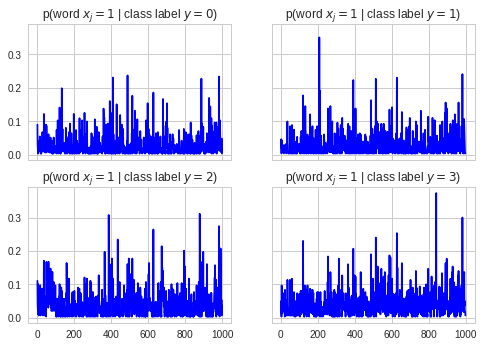
\includegraphics[width=0.45\textwidth]{figures/nb_topics.png}
    \caption{Naive Bayes class-conditional posterior.}
    \label{fig:nb_topics}
\end{figure}

Let's visualize the test document ranking based on entropy and mutual information in Figure \ref{fig:nb_info1}.
\begin{figure}[b]
    \centering
    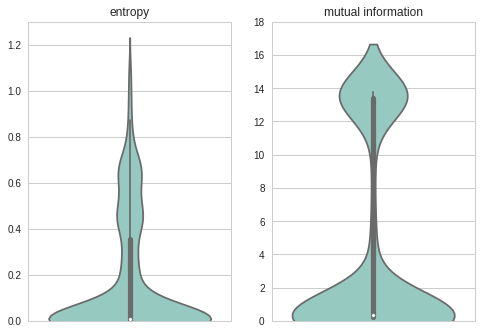
\includegraphics[width=0.45\textwidth]{figures/nb_info1.png}
    \caption{Violin plot showing the density of entropy and MI on test data.}
    \label{fig:nb_info1}
\end{figure}
In particular, we are interested in outliers, i.e. documents that have highest entropy and mutual information. To visualize the difference between entropy and MI based planning, we can sort the documents according to entropy and use the same index to sort MI as shown in Figure \ref{fig:nb_info2}.
\begin{figure}[h]
    \centering
    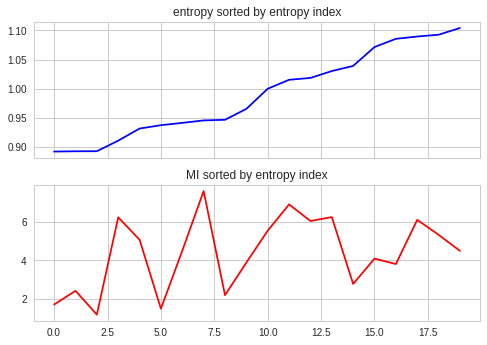
\includegraphics[width=0.45\textwidth]{figures/nb_info2.png}
    \caption{Test document entropy and MI sorted by entropy index.}
    \label{fig:nb_info2}
\end{figure}
In Figure \ref{fig:nb_info2} documents that have high entropy but low MI are uncertain but not informative. Therefore, we expect MI to provide a better measure for information planning.

To evaluate the utility of information planning in comparison to random selection, we take a total of $1K$ documents and divide them into $100$ labelled training documents, $700$ unlabelled test documents, and holdout $200$ documents for evaluating classification performance. We run the active learning pipeline, in which top $K$ most informative documents are selected from the test set, labelled by annotators and added to the training set, at which point the modeled is re-trained from scratch and evaluated on the $200$ heldout documents. Figure \ref{fig:nb_trials_acc} shows the experimental results of this active learning pipeline.
\begin{figure}[h]
    \centering
    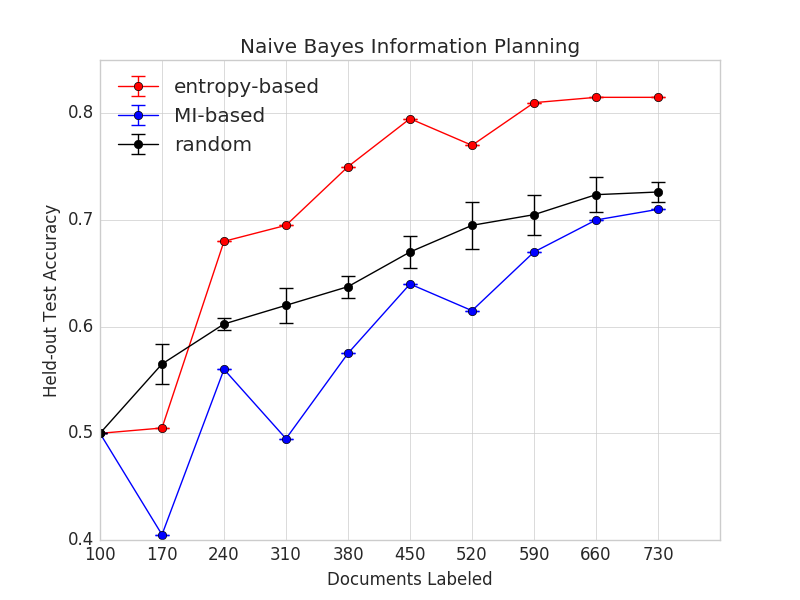
\includegraphics[width=0.45\textwidth]{figures/nb_trials_acc.png}
    \caption{Classification accuracy as a function of labeled examples.}
    \label{fig:nb_trials_acc}
\end{figure}
We can see a clear advantage of using information planning compared to random selection.

\subsection{Supervised LDA}

Latent Dirichlet Allocation (LDA) \cite{Blei2003} is an unsupervised topic model that represents each document as a mixture of topics, where a topic is a distribution over words. The objective is to learn the shared topic distributions and their proportions for each document. However, it is often desirable to associate a quantity of interest (e.g. a score) with each document; this could be a five star rating for a movie review, a quality score of a report, or a number of times an on-line article is linked. Supervised LDA (sLDA) \cite{Blei2010} is designed to jointly learn the topics and the score variable associated with each document. The graphical model of supervised LDA is shown in Figure \ref{fig:slda_gm}. 

\begin{figure}[thpb]
    \centering
    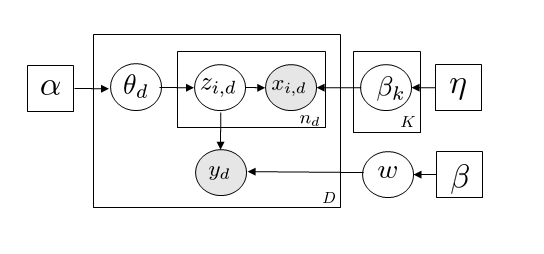
\includegraphics[width=0.45\textwidth]{figures/sLDA_gm.png}
    \caption{Supervised LDA \cite{Blei2010} graphical model.}
    \label{fig:slda_gm}
\end{figure}

sLDA associates each word $x_{id}$ with a topic label $z_{id}\in \{1,...,K\}$. Each document is associated with topic proportions $\theta_d$ that can also be used as a measure of document similarity. The topics $\beta_k$ represented by the Dirichlet distribution are shared across all documents. The hyper-parameters $\alpha$ and $\eta$ capture our prior knowledge of topic proportions and the topics, e.g. from past training of the model. Finally, $y_d$ is the response variable that represents a score associated with each document. In this example, $y_d$ is modelled as a regression between global coefficients $w$ and a normalized histogram of topics present in a document: $\bar{z}$. Assuming a Gaussian distribution, $y_d$ can be expressed as follows:
\begin{eqnarray}
   y_d &\sim& N(w_1\bar{z}_1 + ... + w_k\bar{z}_k, \sigma^2) \\
   \bar{z} &=& \frac{1}{N}\sum_{n=1}^{N}z_n
\end{eqnarray}
where $z_n$ is a one-hot encoded topic assignment vector of size $1\times K$. We use PyMC \cite{PyMC2010} Metropolis-Hastings sampler to infer the latent variables. Figure \ref{fig:slda_topics} shows the first $4$ (out of $8$) topics of sLDA model trained on the polarity sentiment dataset \cite{PolarityDataset}. Notice, that the addition of the score variable $y_d$ influences topic inference due to the coupling between $w$ and $\beta_k$ introduced by the $z_{i,d}\rightarrow y_d \leftarrow w$ and $z_{i,d}\rightarrow x_{i,d} \leftarrow \beta_k$ v-structures \cite{KollerBook}. 
\begin{figure}[h]
    \centering
    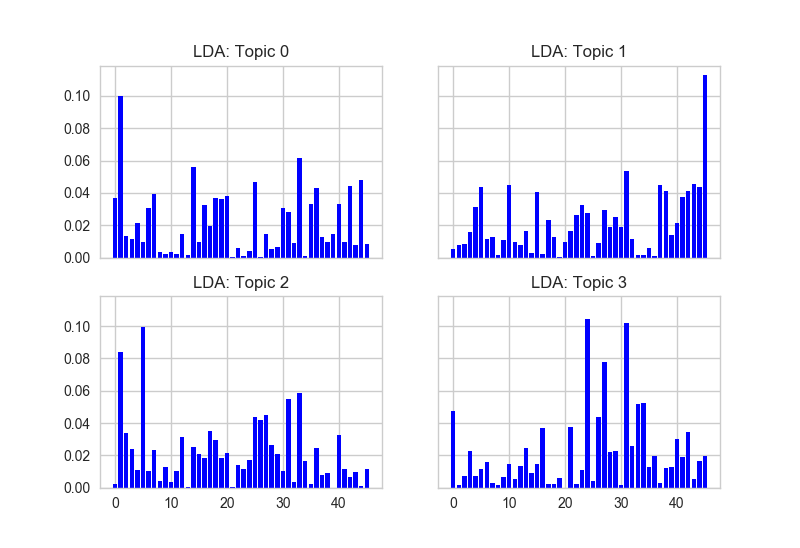
\includegraphics[width=0.45\textwidth]{figures/slda_topics.png}
    \caption{Supervised LDA topics inferred using PyMC \cite{PyMC2010}.}
    \label{fig:slda_topics}
\end{figure}

We can use a sample based estimator to compute the entropy of the score variable $y_d$: $H[y_d|x_d, D] = E[-\log p(y_d|x_d, D)]$.

Assuming we have topic samples:
\begin{equation}
   \{(z_{1d}^{(i)}, ..., z_{Nd}^{(i)})\}_{i=1}^{M} \stackrel{MCMC}{\sim} p(z_{1d},...,z_{Nd}|x_d, D) 
\end{equation}
\begin{equation}
   p(y_d|x_d, D) = \sum_{z_{1d}}...\sum_{z_{Nd}} p(z_{1d},...,z_{Nd}|x_d, D)p(y_d|z_d) \approx \frac{1}{M} \sum_{i=1}^{M}p(y_d|z_d = z_{d}^{(i)}) = \hat{p}(y_d|x_d, D)
\end{equation}
Once we have a sample estimate $\hat{p}(y_d|x_d, D)$, to compute entropy, we need to estimate the expectation:
\begin{equation}
   E[-\log \hat{p}(y_d|x_d,D)] = - \int p(y_d|x_d, D) \log \hat{p}(y_d|x_d, D) dy_d \approx \frac{1}{M}\sum_{i=1}^{M}\log \hat{p}(y_{d}^{(i)}|x_d, D)
\end{equation}
where $\{(y_{d}^{(i)})\}_{i=1}^{M} \stackrel{MCMC}{\sim} \hat{p}(y_{d}^{(i)}|x_d, D)$.

To evaluate the utility of information planning in comparison to random selection, we start with a corpus of $100$ documents, from which we allocate $15$ documents for training, $35$ for testing and holdout $50$ documents for evaluating sLDA performance. Figure \ref{fig:slda_test_mse} shows the test MSE of the Gaussian score variable evaluated against the ground truth review score on the heldout set of $50$ documents.

\begin{figure}[thpb]
    \centering
    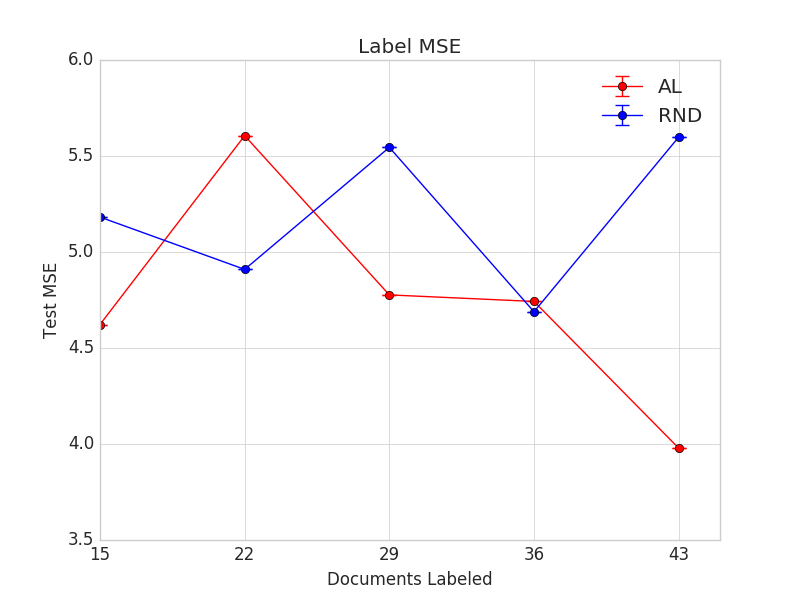
\includegraphics[width=0.4\textwidth]{figures/slda_test_mse.png}
    \caption{Supervised LDA test MSE.}
    \label{fig:slda_test_mse}
\end{figure}

We can see that active learning selection achieves smaller MSE in comparison to random selection baseline.

\subsection{Deep Neural Network}

We consider information planning in the case of deep neural networks. In particular, we examine two architectures: LSTM and CNN in application to sentence sentiment classification \cite{DLBook}. 

Recurrent Neural Networks (RNNs) provide a natural way of encoding a sentence as a sequence of words. Just as you are processing this sentence word by word while keeping a memory of what came before, RNNs maintain an internal model of the past and update it as soon as the new information arrives. Thus, RNNs contain an internal loop unrolled over the length of the input sequence. As a result, RNNs can capture more information in comparison to $n$-gram models. For example, in a $n$-gram language model (with $n=3$), we can predict the next word given the previous two:
\begin{equation}
    l_{sent} = \frac{1}{n}\log P(w_1,...,w_n) = \frac{1}{n}\sum_{i=1}^{n}\log p(w_i|w_{i-1}, w_{i-2})
\end{equation}
The dependence in neural language model (LM) extends to the beginning of the sentence, i.e. $p(w_{i}|w_{i-1},...,w_1)$, while in a $n$-gram LM the conditioning is only on the previous $n$ words and as $n$ grows larger, sparsity of training data becomes a problem. In both cases, the word conditional distribution greatly reduces the output space of possible words and enables learning of word representations based on their context \cite{word2vec2013}.    

\begin{table*}[t]
\centering
\begin{tabularx}{\linewidth}{XX}
    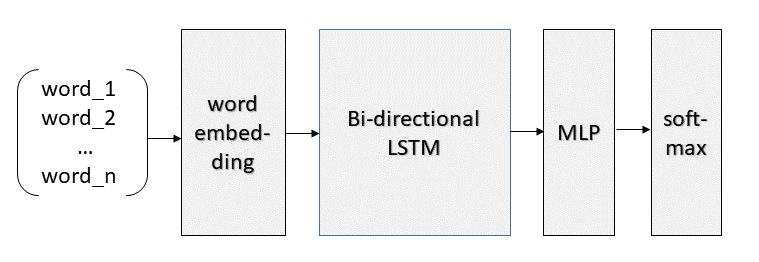
\includegraphics[width=0.5\columnwidth]{./figures/lstm_architecture.png}
    \captionof{figure}{LSTM model architecture}
    \label{fig:lstm_arch}
&
    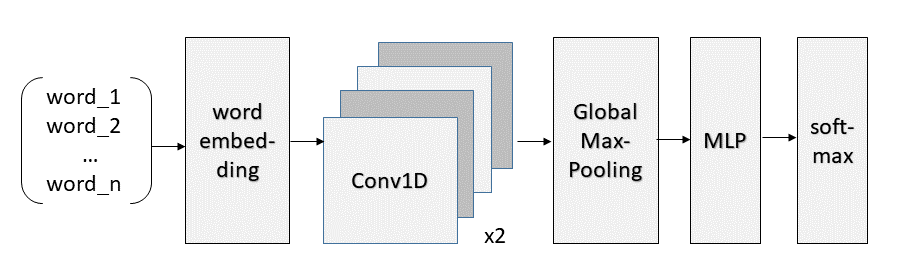
\includegraphics[width=0.5\columnwidth]{./figures/cnn_architecture.png}
    \captionof{figure}{CNN model architecture}
    \label{fig:cnn_arch}
\\
\end{tabularx}
\end{table*}

A sentence can be encoded by an RNN (such as LSTM) as either the output of its last layer or via average pooling of its intermediate outputs. In both cases, the word position information is preserved in contrast to averaging of word vectors. Figure \ref{fig:lstm_arch} shows the LSTM architecture used for sentiment classification. We use a bi-directional LSTM that concatenates sequence representations of forward and reverse LSTMs. This enriches order-sensitive representation of the sentence and leads to a slight increase in accuracy. In addition to output layer dropout, we use recurrent dropout that applies the same dropout mask at every time-step (in contrast to a dropout mask that varies randomly between time-steps that could harm the learning process) \cite{Gal2016}.   

Convolutional Neural Networks (CNNs) offer computational advantages due to their parallel nature and comparable performance with time-series data, especially in cases when recent past is not more informative than the distant past (due to translation invariance of CNNs). The same properties that make convnets excel at computer vision also make them highly relevant for sequence processing. Time can be treated as a spatial dimension like the height or width of a 2D image. For example, 1D convolutions can be used to extract patterns from local 1D patch sub-sequences of the input sequence. Because the same transformation is performed on every patch, a pattern learned at a certain position in the sentence can later be recognized at a different position, making 1D convnets translation invariant. While a word-level conv-net operating on word embeddings with a kernel size of $5$ should be able to recognize words or word fragments of length $5$ or less, a character-level 1D conv-net is able to learn about word morphology. In addition, we can learn hierarchical patterns by stacking several convolutional layers. Figure \ref{fig:cnn_arch} shows the CNN architecture used for sentiment classification. It consists of a word embedding layer followed by a stack of two convolutional layers separated by a dropout layer. Finally, the activations across each of the filters are pooled via global max pooling and fed into a Multi-Layer Perceptron (MLP) classifier.  

For both LSTM and CNN models, we choose pre-trained word embeddings because in an active learning setting, there's usually not enough training data to learn specialized word embeddings for a given task. In order to preserve the latent structure (that could otherwise be destroyed by large gradients from randomly initialized downstream layers), we configure the embeddings to be non-trainable. Both architectures use Glove pre-trained word embeddings \cite{Glove2014} based on word co-occurence for dense representation of words. 

As shown in \cite{MCDropout2016} dropout \cite{Dropout2014} and other stochastic regularization techniques can be used for approximate inference in deep neural networks. This is accomplished by using dropout at test-time and computing Monte Carlo integration (referred to as MC dropout):
\begin{eqnarray}
    &&p(y=c|x, D) = \int p(y=c|x, w)p(w|D)dw \\ 
    &&\approx \int p(y=c|x,w)q_{\theta}^{\ast}(w)dw \approx \frac{1}{T}\sum_{t=1}^{T}p(y=c|x,\hat{w}_t) \nonumber
\end{eqnarray}
where $\hat{w}_{t} \sim q_{\theta}^{\ast}(w)$ and $q_{\theta}^{\ast}(w)$ is a variational distribution that minimizes KL divergence to the true model posterior $p(w|D)$:
\begin{equation}
    \arg \min_{\theta} KL(q_{\theta}(w) || p(w|D))
\end{equation}
where $\theta$ are the variational parameters and $w$ are the neural network weights. Averaging forward passes with MC dropout during test time is equivalent to Monte Carlo integration over a Gaussian process posterior approximation \cite{Gal2017}. 

We consider two acquisition functions: one based on entropy and one based on mutual information. An \textit{acquisition function} $a(x,M)$ determines which measurements to take next, and it's a function of the pool of unlabelled examples $x \in D_{pool}$ and the model $M$:
\begin{equation}
    x^{\ast} = \arg \max_{x \in D_{pool}} a(x,M)
\end{equation}
In the case of entropy, we want to choose data points that maximize:
\begin{equation}
    H[y|x, D] = -\sum_{c}p(y=c|x,D)\log p(y=c|x,D)
\end{equation}
In the case of mutual information, we want to choose data points that maximize the information gain between the predictions $y$ and the model parameters $w$:
\begin{equation}
    I(y;w|x,D) = H[y|x, D] - E_{p(w|D)}[H[y|w,x,D]]
\end{equation}
where $w$ in our case are the weights of the neural network and the expectation is computed using MC dropout. Thus, we are seeking data points $x$ for which the model is both marginally most uncertain about $y$ and most confident about the predicted label. Notice, that it's easier to compute MI as written above (as opposed to its alternative version) because the entropies are computed in a discrete, low-dimensional output space. This interpretation allows reasoning about uncertainty in deep learning and the application of Bayesian methods to analyze existing deep learning frameworks. 

We evaluate the effectiveness of information planning on Kaggle movie review sentiment dataset 
\cite{KaggleSentiment}. The dataset consists of phrases from the Rotten Tomatoes dataset classified into $5$ sentiment labels: negative, somewhat negative, neutral, somewhat positive and positive. Obstacles such as sentence negation, sarcasm, and language ambiguity make this a challenging task. We take the first 10K sentences, set aside 10\% for training and holdout 10\% for evaluating the performance. At each iteration, we select the top $K=800$ most informative sentences to be annotated and added to the training set. Figures \ref{fig:cnn_acc_trials}, \ref{fig:cnn_entropy_trials}, \ref{fig:lstm_acc_trials}, \ref{fig:lstm_entropy_trials} show active learning experimental results.

\begin{table*}[t]
\centering
\begin{tabularx}{\linewidth}{XXXX}
    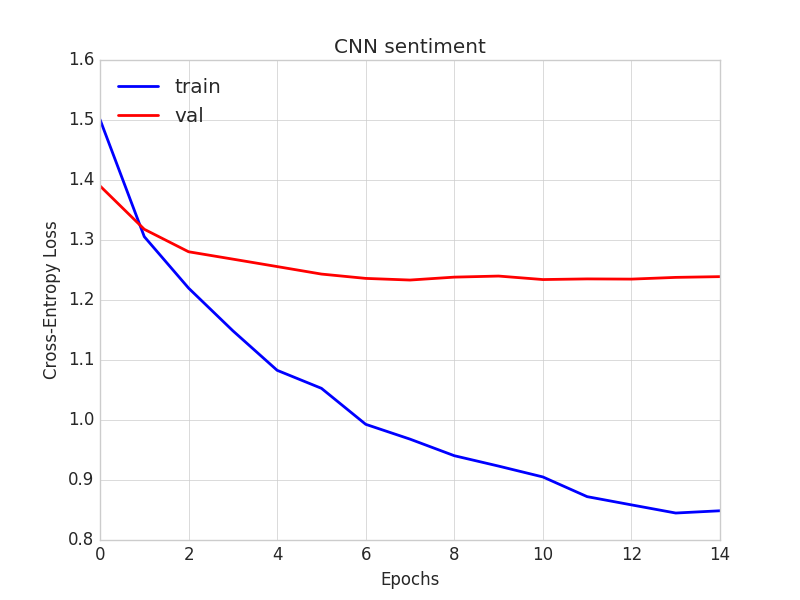
\includegraphics[width=0.25\columnwidth]{./figures/cnn_sentiment_loss.png}
    \captionof{figure}{CNN: training loss}
    \label{fig:cnn_loss}
&
    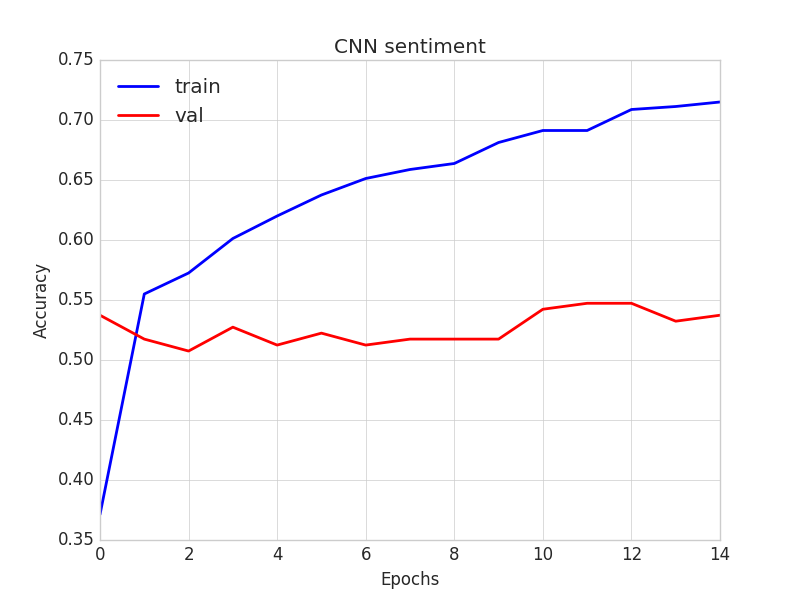
\includegraphics[width=0.25\columnwidth]{./figures/cnn_sentiment_acc.png}
    \captionof{figure}{CNN: training acc}
    \label{fig:cnn_acc}
&
    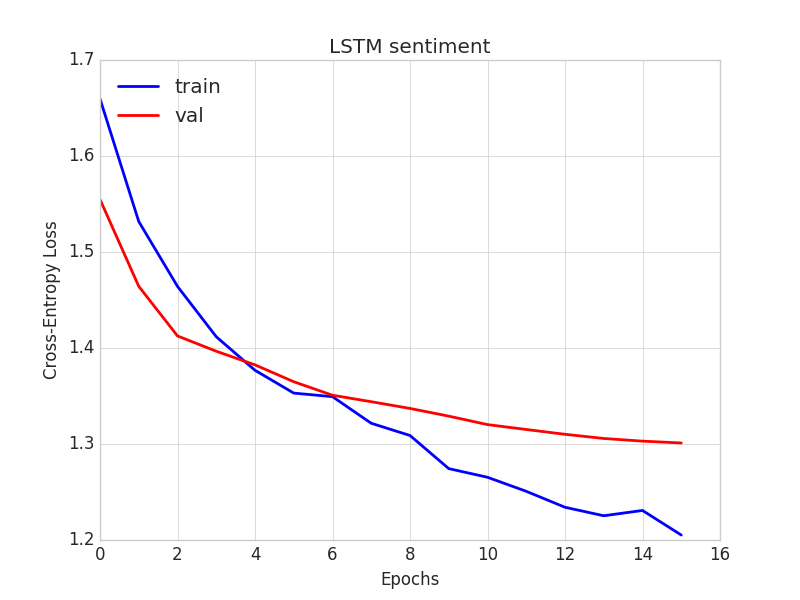
\includegraphics[width=0.25\columnwidth]{./figures/lstm_sentiment_loss.png}
    \captionof{figure}{LSTM: training loss}
    \label{fig:lstm_loss}
&
    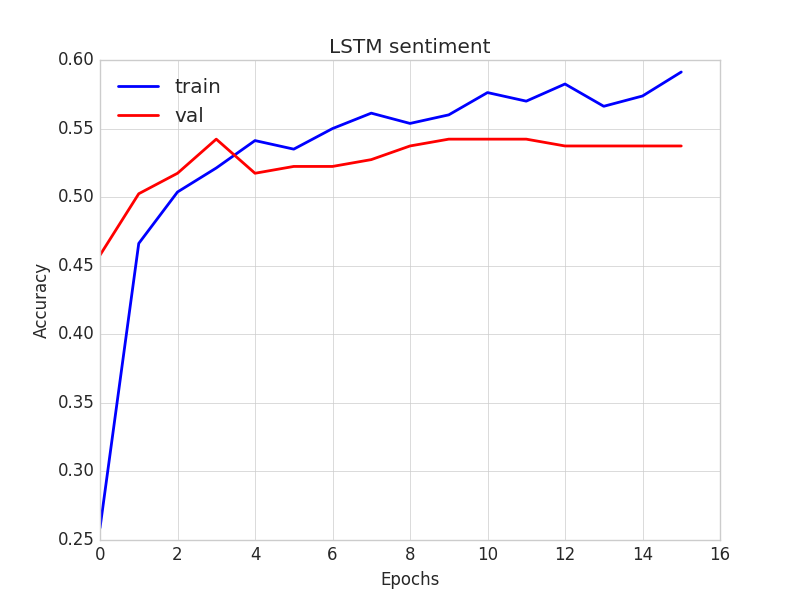
\includegraphics[width=0.25\columnwidth]{./figures/lstm_sentiment_acc.png}
    \captionof{figure}{LSTM: training acc}
    \label{fig:lstm_acc}
\\
\end{tabularx}
\end{table*}
   
\begin{table*}[t]
\centering
\begin{tabularx}{\linewidth}{XXXX}
    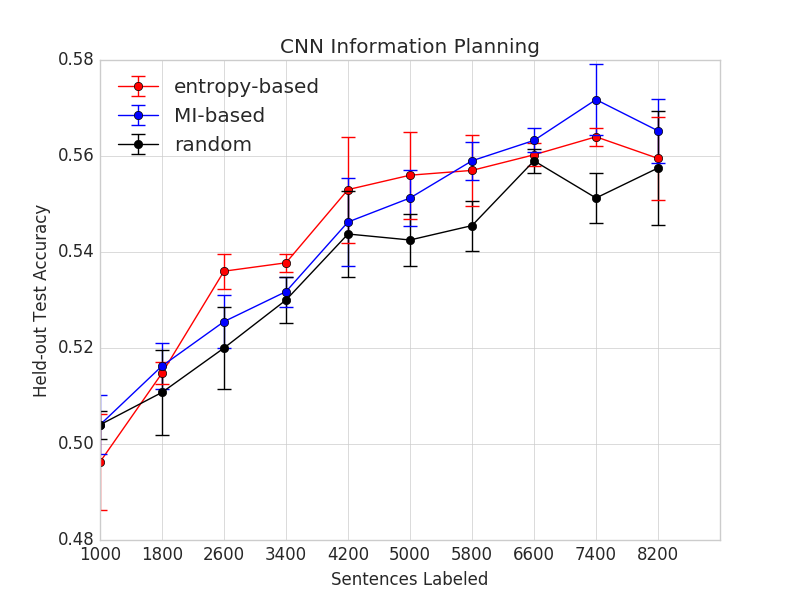
\includegraphics[width=0.25\columnwidth]{./figures/cnn_sentiment_trials_accuracy.png}
    \captionof{figure}{CNN: test accuracy}
    \label{fig:cnn_acc_trials}
&
    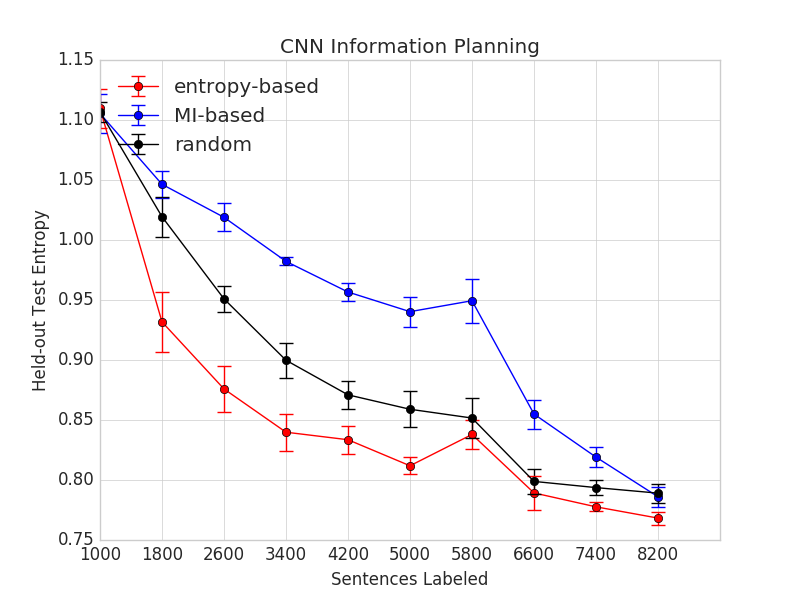
\includegraphics[width=0.25\columnwidth]{./figures/cnn_sentiment_trials_entropy.png}
    \captionof{figure}{CNN: test entropy}
    \label{fig:cnn_entropy_trials}
&
    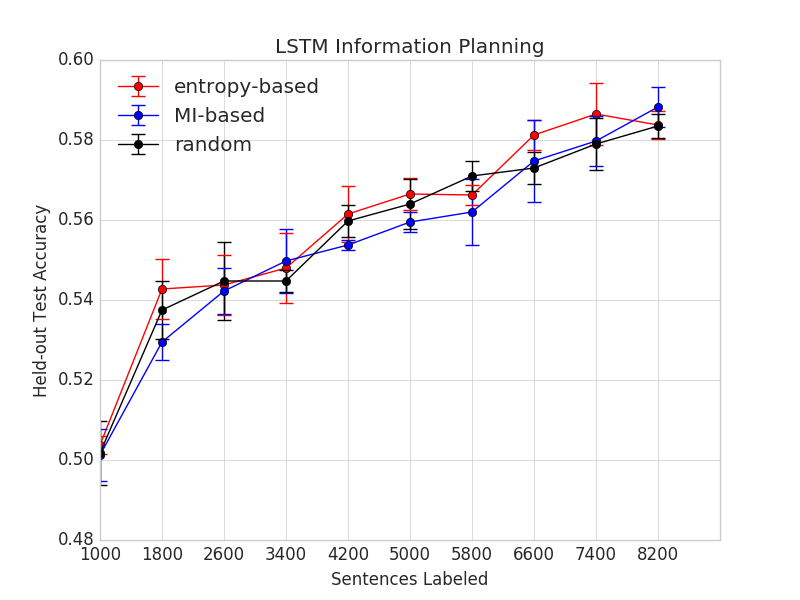
\includegraphics[width=0.25\columnwidth]{./figures/lstm_sentiment_trials_accuracy.png}
    \captionof{figure}{LSTM: test acc.}
    \label{fig:lstm_acc_trials}
&
    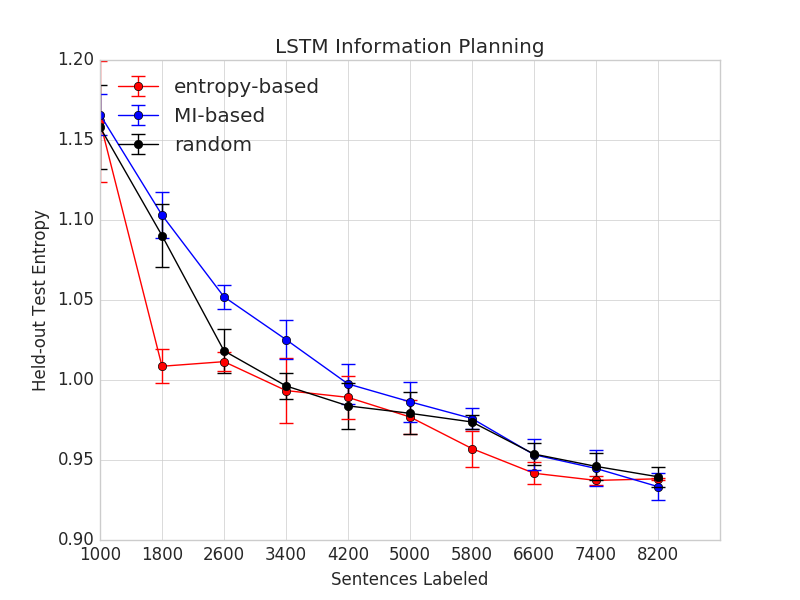
\includegraphics[width=0.25\columnwidth]{./figures/lstm_sentiment_trials_entropy.png}
    \captionof{figure}{LSTM: test entropy}
    \label{fig:lstm_entropy_trials}
\\
\end{tabularx}
\end{table*}
   
\subsection{Discussion}
In this section we discuss information planning results for each model.

Naive Bayes is the simplest model for studying information planning since all latent variables are discrete and information measures can be computed in closed form. By choosing the Bernoulli formulation of Naive Bayes we were able to do planning at the word level. In particular, the top-10 highest MI words as shown in Table \ref{tab:nb_words} were found to be informative of the ground truth labels.  
\begin{table}[h]
\begin{center}
  \begin{tabular}{c|c|c|c|c}
    \toprule
    class 0 & class 1 & class 2  & class 3 & MI       \\ \midrule
    get     & think   & first    & nasa    & teams    \\
    please  & well    & time     & could   & program  \\
    use     & know    & season   & much    & league   \\
    like    & also    & year     & know    & moon     \\
    one     & cars    & play     & get     & playoffs \\
    anyone  & get     & hockey   & also    & orbit    \\
    thanks  & like    & one      & like    & players  \\
    graphics& one     & would    & one     & earth    \\
    would   & would   & game     & would   & games    \\
    know    & car     & team     & space   & nasa     \\
    \bottomrule
  \end{tabular}
\end{center}
\caption{Naive Bayes: top 10 words. Ground truth labels: graphics, autos, hockey, space.}
\label{tab:nb_words}
\end{table}

From Figure \ref{fig:nb_trials_acc}, we can see that we achieve about $10\%$ accuracy increase when we use uncertainty sampling in comparison to random selection. All experimentes were repeated $10$ times.  

In supervised LDA model, the score variable is learned jointly with the topics. Figure \ref{fig:slda_test_mse} shows that smaller MSE is achieved with uncertainty sampling in comparison to random selection. We also note that sampling based inference for sLDA is more suitable to stream queres in which documents are queried one at a time due considerable time it takes to run sampling for the entire pool of unlabelled examples. 

In deep neural network setting we assume that computational expense of re-training the model from scratch is justified by the cost of obtaining the labels. From the training and validation loss in Figures \ref{fig:cnn_loss}, \ref{fig:lstm_loss}, we see no signs of over-fitting due regularization with dropout and weight decay. The validation loss plateaus early in the training indicating that model capacity can be increased in an attempt to achieve higher classification accuracy. Figures \ref{fig:cnn_acc}, \ref{fig:lstm_acc} show that CNN and LSTM model achieve comparable accuracy on the sentiment classification task with validation accuracy close to $55\%$.     

Figures \ref{fig:cnn_acc_trials}, \ref{fig:lstm_acc_trials} show the benefit of information planning over the random basline. We can see that we achieve close to $1\%$ improvement in accuracy in the case of CNN and a relatively smaller improvement in the case of LSTM, even thought LSTM achieves $2\%$ higher held-out test accuracy in the end. It's also interesting to see, the decrease in test label entropy as shown in Figures \ref{fig:cnn_entropy_trials}, \ref{fig:lstm_entropy_trials}, where as expected the uncertainty sampling leads to highest reduction in entropy. 
 


\newpage
\section{Misc}
\subsection{Sequential Monte Carlo}

Particle Filters (PF) is a Sequential Monte Carlo (SMC) method for estimating the internal states of a Switching Linear Dynamic System (SLDS). A set of particles is used to represent the posterior distribution of the states of the Markov process. At each iteration, the particles get re-samples and the ones that explain the observations best survive to the next iteration.

The Gaussian SLDS can be described as follows \cite{deFreitas2002}:
\begin{eqnarray}
    z_t &\sim& P(z_t | z_{t-1})\\
    x_t &=& A(z_t)x_{t-1} + B(z_t)w_t + F(z_t)u_t \\
    y_t &=& C(z_t)x_t + D(z_t)v_t + G(z_t)u_t
\end{eqnarray}
where $y_t \in \mathbb{R}$ denotes the observations, $x_t \in \mathbb{R}$ denotes latent Gaussian states, $z_t \in \mathbb{Z}$ denotes latent discrete states and $u_t$ is a known control signal. The noise processes are iid Gaussian with $w_t \sim N(0,I)$ and $v_t \sim N(0,I)$. This model implies the continuous densities:
\begin{eqnarray}\label{equ:smc_density}
    p(x_t|z_t,x_{t-1}) &\sim& N(A(z_t)x_{t-1} + F(z_t)u_t, B(z_t)B(z_t)^{T})\\
    p(y_t|x_t,z_t) &\sim& N(C(z_t)x_t + G(z_t)u_t, D(z_t)D(z_t)^{T})
\end{eqnarray}
along with initial states $x_0 \sim N(\mu_0,\Sigma_0)$ and $z_0 \sim P(z_0)$. The aim of the analysis is to compute the marginal posterior distribution of the discrete states $p(z_{0:t}, y_{1:t})$. The posterior density can be factorized as follows:
\begin{equation}
    p(x_{1:t},z_{1:t}|y_{1:t}) = p(x_{1:t}|y_{1:t},z_{1:t})p(z_{1:t}|y_{1:t})
\end{equation}
where the density $p(x_{1:t}|y_{1:t},z_{1:t})$ is Gaussian and can be computed analytically if we know the marginal posterior density $p(z_{1:t}|y_{1:t})$. We can re-write the marginal posterior recursively:
\begin{eqnarray}
   p(z_{1:t}|y_{1:t}) &=& \frac{p(y_t|z_{1:t}, y_{1:t-1})p(z_{1:t}|y_{1:t-1})}{p(y_t|y_{1:t-1})}\\
   &=& \frac{p(y_t|z_t)p(z_t|z_{1:t-1},y_{1:t-1})p(z_{1:t-1}|y_{1:t-1})}{p(y_t|y_{1:t-1})}\\
   &\propto& p(y_t|z_t)p(z_t|z_{t-1})p(z_{1:t-1}|y_{1:t-1})
\end{eqnarray}
which depends only on the current conditional distributions and previously computed $p(z_{1:t-1}|y_{1:t-1})$. The basic idea is to approximate the belief state of the entire state trajectory using a weighted set of particles:
\begin{equation}
    p(z_{1:t}|y_{1:t}) \approx \sum_{s=1}^{S}\hat{w}_{t}^{s}\delta_{z_{1:t}^{s}}(z_{1:t})
\end{equation}
We update this belief using importance sampling. If the proposal has the form $q(z_{1:t}^{s}|y_{1:t})$ then the importance weights are given by:
\begin{equation}
    w_{t}^{s} \propto \frac{p(z_{1:t}^{s}|y_{1:t})}{q(z_{1:t}^{s}|y_{1:t})} \propto \frac{p(y_t|x_t,z_t)p(x_t, z_t|x_{t-1},z_{t-1})}{q(x_t,z_t|x_{t-1},z_{t-1})} 
\end{equation}
We can choose the transition prior to be the proposal distribution:
\begin{equation}
     q(x_t,z_t|x_{t-1},z_{t-1}) = p(x_t, z_t|x_{t-1},z_{t-1}) = p(x_t|x_{t-1},z_{t-1})p(z_t|z_{t-1})
\end{equation}
then the importance weights are given by the likelihood function: $w_t \propto p(y_t|x_t,z_t)$. The particle filter algorithm is summarized in Algorithm \ref{alg:pf}.

\begin{algorithm}
\caption{Particle Filter Algorithm \cite{deFreitas2002}}
\label{alg:pf}
\begin{algorithmic}[1]
\STATE \textit{Sequential Importance Sampling Step}
\STATE for i = 1 to $N$ do  
\STATE ~~~ $z_{t}^{i} \sim p(z_t|z_{t-1}^{i})$ 
\STATE ~~~ $x_{t}^{i} \sim p(x_t|x_{t-1}^{i}, z_{t}^{i})$ as in eq. (\ref{equ:smc_density})
\STATE end for 
\STATE for i = 1 to $N$ do 
\STATE ~~~ $w_{t}^{i} \propto p(y_t|x_{t}^{i}, z_{t}^{i})$
\STATE end for
\STATE $\hat{w}_{t}^{i} = \frac{w_{t}^{i}}{\sum_{s^{\prime}}w_{t}^{s^{\prime}}}$ 
\STATE \textit{Selection Step}
\STATE ~~~ Multiply particles with respect to importance weights $w_{t}^{i}$
\STATE ~~~ to obtain $N$ particles $\{x_{1:t}^{i},z_{1:t}^{i}\}_{i=1}^{N}$
\STATE end for
\end{algorithmic}
\end{algorithm}

The selection step modifies the weighted approximate density $p_N$ to an unweighted density $\hat{p}_N$ by eliminating particles with low importance weights and by multiplying particles with high importance weights. Thus, $p_N(x)=\sum_{i=1}^{N}w_i\delta(x-x_i)$ is replaced by
\begin{equation}
    \hat{p}_N(x) = \sum_{k=1}^{N}\frac{1}{N}\delta(x-x_{k}^{\ast}) = \sum_{i=1}^{N}\frac{n_i}{N}\delta(x-x_i)
\end{equation}
There are many resampling schemes such as multinomial, stratified, systematic and residual.
All these algorithms are unbiased and can be implemented in $O(N)$ time.\\

The Rao-Blackwellized Particle Filter (RBPF) is similar to the PF but we only sample the discrete states. Then for each sample of the discrete states, we update the mean and covariance of the continuous states using Kalman filter updates. In particular, we sample $z_{t}^{i}$ and then propagate the mean $\mu_{t}^{i}$ and covariance $\Sigma_{t}^{i}$ of $x_t$ with a Kalman filter as follows:
\begin{eqnarray}
\mu_{t|t-1}^{i} &=& A(z_{t}^{i})\mu_{t-1|t-1}^{i} + F(z_{t}^{i})u_t\\
\Sigma_{t|t-1}^{i} &=& A(z_{t}^{i})\Sigma_{t-1|t-1}^{i}A(z_{t}^{i})^{T} + D(z_{t}^{i})D(z_{t}^{i})^{T}\\
S_{t}^{i} &=& C(z_{t}^{i})\Sigma_{t|t-1}^{i}C(z_{t}^{i})^{T} + D(z_{t}^{i})D(z_{t}^{i})^{T}\\
y_{t|t-1}^{i} &=& C(z_{t}^{i})\mu_{t|t-1}^{i} + G(z_{t}^{i})u_t\\
\mu_{t|t}^{i} &=& \mu_{t|t-1}^{i} + \Sigma_{t|t-1}^{i}C(z_{t}^{i})^{T}S_{t}^{-1}(y_t - y_{t|t-1}^{i})\\
\Sigma_{t|t}^{i} &=& \Sigma_{t|t-1}^{i} - \Sigma_{t|t-1}^{i}C(z_{t}^{i})^{T}S_{t}^{-1}C(z_{t}^{i})\Sigma_{t|t-1}^{i}
\end{eqnarray}

The RBPF takes slightly longer to compute but results in more accurate predictions. Figure \ref{fig:pf_merged} shows the generated SLDS states (left) and the inferred states (middle) by Particle Filter (PF) and the Rao-Blackwellized version (RBPF).
\begin{figure}[tbhp]
    \centering
    \includegraphics[width=0.9\textwidth, trim={10 10 10 10}]{figures/particle_filter_merged.png}
    \caption{Particle Filter inference using PF and RBPF applied to Switching Linear Dynamic System.}
    \label{fig:pf_merged}
\end{figure}
We can see that the inferred states closely correspond to the ground truth. Also shown is a particle resampling step (right) where only a fraction of the particles survive to the next iteration.


\subsection{Information Theory}

Information theory addresses the problems of data representation and reliable transmission of information. In order to measure information content, we define several information measures below.

\subsubsection{Entropy}

The entropy of a random variable is a measure of its uncertainty. Let $X$ be a discrete random variable with probability mass function $p(x)$, then its entropy is defined as:
\begin{equation}
    H(X) = -\sum_{x} p(x) \log p(x) = -E[\log p(x)]
\end{equation}
A maximum entropy discrete distribution is the uniform distribution. For a random variable with support $K$ and $p(x)=1/K$, the entropy is $H(X)= -\sum \frac{1}{K} \log \frac{1}{K} = \log_2 K$. Thus, entropy is measured in bits (using log base 2) or nats (using log base $e$). In contrast, the entropy of a deterministic random variable with $p(x) = \delta[x]$ is $H(X) = 1\log 1 = 0$. In the special case of a binary random variable $X \in \{0,1\}$ with $p(x=1)=p$, the entropy is
\begin{equation}
    H(X) = -p \log p - (1-p)\log (1-p)
\end{equation}
It is a concave function with maximum uncertainty of $1$ bit occuring at $p=\frac{1}{2}$, when $p=0$ or $p=1$, the entropy is $0$. Since entropy is a concave function on the space of distributions, we have:
\begin{equation}
    H(\lambda p_1 + (1-\lambda) p_2) \geq \lambda H(p_1) + (1-\lambda) H(p_2)
\end{equation}
\textit{Proof.} To prove that $H(p)$ is concave at $p$, we can use the log-sum inequality. Let $p_\lambda(y) = \lambda p_1(y) + (1-\lambda)p_2(y)$then,
\begin{eqnarray}
    -H(p_\lambda) &=& \sum_y p_\lambda(y) \log p_\lambda(y) \\ \nonumber
    &=& \sum_y \big[\lambda p_1(y) + (1-\lambda)p_2(y)\big] \log \big[\lambda p_1(y) + (1-\lambda)p_2(y) \big]
\end{eqnarray}
Let's use the log-sum inequality with $K=2$ and $a_1 = \lambda p_1(y)$, $a_2 = (1-\lambda)p_2(y)$, $b_1 = \lambda$ and $b_2 = (1-\lambda)$:
\begin{eqnarray}
    -H(p_\lambda) &\leq& \lambda p_1(y)\log \frac{\lambda p_1(y)}{\lambda} + (1-\lambda)p_2(y)\log \frac{(1-\lambda)p_2(y)}{1-\lambda} \\ \nonumber
    &=& \lambda p_1(y)\log p_1(y) + (1-\lambda)p_2(y)\log p_2(y) \\ \nonumber
    &=& -\big[\lambda H(p_1) + (1-\lambda)H(p_2)\big]
\end{eqnarray}


Since $0\leq p(x) \leq 1$, we have $\log \frac{1}{p(x)} \geq 0$, and for a discrete $X$, the entropy is non-negative: $H(X)\geq 0$. We can find an upper bound for entropy using the Jensen's inequality:
\begin{eqnarray}
    H(X) &=& \sum_{x \in \cal X} p(x)\log \frac{1}{p(x)} \\
         &\leq& \log \sum_{x \in \cal X} p(x)\times \frac{1}{p(x)} \\
         &=& \log \sum_{x \in \cal X} 1 \\
         &=& \log |\cal X|
\end{eqnarray}
We also note that entropy is independent of permutation or cyclical shifts of the support of our distribution, i.e. it only depends on the point masses $p(x)$.\\

The joint entropy of a pair of discrete random variables $X$ and $Y$ is defined as:
\begin{equation}
    H(X,Y) = -\sum_x \sum_y p(x,y) \log p(x,y) = -E[\log p(x,y)]
\end{equation}
when two variables are independent the joint entropy is additivie: $H(X,Y) = H(X) + H(Y)$ iff $p(x,y) = p(x)p(y)$. The conditional entropy is defined as:
\begin{eqnarray}
    H(X|Y) &=& \sum_y p(y)H(X|Y=y) = -\sum_y p(y)\sum_x p(x|y)\log p(x|y) \\
           &=& -\sum_x \sum_y p(x,y)\log p(x|y) = -E[\log p(x|y)]
\end{eqnarray}
Note that conditioning on $Y$ the uncertainty over $X$ reduces on average: $H(X|Y) \leq H(X)$. The entropy of a pair of variables follows the chain rule:
\begin{eqnarray}
    H(X,Y) = H(X) + H(Y|X) = H(Y) + H(X|Y)
\end{eqnarray}
which follows from the chain rule for probability: $p(x,y) = p(x)p(y|x) = p(y)p(x|y)$. The chain rule can be generalized for multiple random variables $X_1,...,X_N$:
\begin{equation}
    H(X_1,...,X_N) = \sum_{i=2}^{N}H(X_i|X_1,...,X_{i-1}) + H(X_1) \leq \sum_{i=1}^{N} H(X_i)
\end{equation}
where the inequality follows from the fact that conditioning reduces entropy. For continuous random variables, the multivariate Gaussian is the distribution with maximum differential entropy:
\begin{eqnarray}
    h(X_1,...,X_n) &=& \int p(x) \log \frac{1}{p(x)} dx \\
    &=& \int p(x) \bigg[\frac{1}{2}\log (2\pi)^{n}|\Sigma| + \frac{1}{2}(x-\mu)^{T}\Sigma^{-1}(x-\mu)\bigg] dx \\
    &=& \frac{1}{2}\log (2\pi)^{n}|\Sigma| + \frac{1}{2}E[(x-\mu)^{T}\Sigma^{-1}(x-\mu)] \\
    &=& \frac{1}{2}\log (2\pi)^{n}|\Sigma| + \frac{1}{2}Tr\{\Sigma^{-1}\Sigma\} \\
    &=& \frac{1}{2}\log (2\pi)^{n}|\Sigma| + \frac{1}{2}n \log e = \frac{1}{2}\log\big[(2\pi e)^n|\Sigma|\big] 
\end{eqnarray}
In information theory, the analog of the law of large numbers is the Asymptotic Equipartition Property (AEP). The AEP states that:
\begin{theorem}
(AEP) If $X_1$,$X_2$,...,$X_n$ are iid $\sim p(x)$ then
\begin{equation}
    -\frac{1}{n} \log p(X_1, X_2,...,X_n) \rightarrow H(X) ~~~\mathrm{in~probability}
\end{equation}
\end{theorem}
\textit{Proof}.
\begin{equation}
    -\frac{1}{n}\log p(X_1, X_2,...,X_n) = -\frac{1}{n}\sum_i \log p(X_i) \rightarrow -E[\log p(X)] = H(X)
\end{equation}
Thus, the probability $p(X_1,...,X_n)$ assigned to an observed sequence will be close to $2^{-nH(X)}$. This enables us to classify the set of all sequences into a typical set, where the sample entropy is close to the true entropy and the nontypical set that contains all other sequences. 

\subsubsection{KL divergence}

One way to measure the similarity between two probability distributions $p(x)$ and $q(x)$ is the Kullback-Leibler divergence or relative entropy. It is defined as follows:
\begin{equation}
    KL(p||q) = \sum_x p(x) \log \frac{p(x)}{q(x)}
\end{equation}
we can re-write it as:
\begin{equation}
    KL(p||q) = \sum_x p(x)\log p(x) - \sum_x p(x)\log q(x) = -H(p) + H(p,q)
\end{equation}
where $H(p,q)$ is the cross-entropy. The regular entropy can be written as $H(p,p)$ and therefore KL divergence can be seen as a penalty of extra bits needed to encode the data due to the fact that we used a distribution $q(x)$ to represent the data instead of the true distribution $p(x)$. 
\begin{theorem}
 (Information Inequality) $KL(p||q)\geq 0$ with equality iff $p = q$. 
\end{theorem}
\textit{Proof}.
\begin{eqnarray}
    -KL(p||q) &=& -\sum_x p(x) \log \frac{p(x)}{q(x)} = \sum_x p(x)\log \frac{q(x)}{p(x)} \\
              &\leq& \log \sum_x p(x) \frac{q(x)}{p(x)} = \log \sum_x q(x)\\
              &\leq& \log 1 = 0
\end{eqnarray}
where we used the Jensen's inequality, which states that for any convex function $f(x)$, we have
\begin{equation}
    f\bigg(\sum_{i=1}^{n}\lambda_i x_i \bigg) \leq \sum_{i=1}^{n} \lambda_i f(x_i)
\end{equation}
where $\lambda_i \geq 0$ and $\sum_{i=1}^{n}\lambda_i = 1$.
However, KL divergence is not a true distance between distributions because it is not symmetric ($KL(p||q) \neq KL(q||p))$ and it does not satisfy the triangle inequality. We can use the information inequality to derive an upper bound on entropy. Let $u(x) = 1/|\cal X|$ be the uniform distribution, then:
\begin{eqnarray}
    0 &\leq& KL(p||u) = \sum_x p(x)\log \frac{p(x)}{u(x)} \\
      &=& \sum_x p(x)\log p(x) - \sum_x p(x)\log u(x) \\
      &=& -H(X) + \log |\cal X|
\end{eqnarray}
Thus, $H(X) \leq \log |\cal X|$ with equality iff $p(x) = u(x)$. 

Before discussing the structure / properties of $D(p||q)$, it's helpful to introduce the log-sum inequality.
\begin{theorem}
Let $a_1,...,a_n$ and $b_1,...,b_n$ be non-negative numbers. Let $a = \sum_{i=1}^{n}a_i$ and $b = \sum_{i=1}^{n}b_i$ then
\begin{equation}
    \sum_{i=1}^{n}a_i\log \frac{a_i}{b_i} \geq a \log \frac{a}{b}
\end{equation}
with equality iff $\frac{a_i}{b_i}$ are equal for all $i$.
\end{theorem}
\textit{Proof}. Let's define $f(x) = x\log x$, notice that $f(x)$ is convex (since $f^{\prime \prime}(x) = \frac{1}{x} > 0$ for $x > 0$). Then, we have:
\begin{eqnarray}
    \sum_{i=1}^{n} a_i \log \frac{a_i}{b_i} &=& \sum_{i=1}^{n}b_i f(\frac{a_i}{b_i}) = b \sum_{i=1}^{n}\frac{b_i}{b}f(\frac{a_i}{b_i}) \\ \nonumber
    &\geq& bf\bigg(\sum_{i=1}^{n}\frac{b_i}{b}\frac{a_i}{b_i}\bigg) = bf\bigg(\frac{1}{b}\sum_{i=1}^{n}a_i \bigg) = bf\big(\frac{a}{b}\big) \\ \nonumber 
    &=& a \log \frac{a}{b}
\end{eqnarray}

\begin{theorem}
   $KL(p||q)$ is convex in the pair $(p,q)$, i.e.
   \begin{equation}
        KL(\lambda p_1 + (1-\lambda)p_2 || \lambda q_1 + (1-\lambda) q_2) \leq \lambda KL(p_1||q_1) + (1-\lambda) KL(p_2||q_2)
   \end{equation}
\end{theorem}
\textit{Proof}. Expanding the inequality above, we want to show that
\begin{eqnarray}
\sum_x(\lambda p_1(x) + (1-\lambda)p_2(x))\log\frac{\lambda p_1(x) + (1-\lambda)p_2(x)}{\lambda q_1(x) + (1-\lambda)q_2(x)} \leq \\
\lambda \sum_x p_1(x)\log\frac{p_1(x)}{q_1(x)} + (1-\lambda)\sum_x p_2(x)\log\frac{p_2(x)}{q_2(x)}
\end{eqnarray}
Then for a fixed $x$, it suffices to show that
\begin{equation}
    \sum_{i=1,2} \lambda_i p_i \log \frac{\lambda_i p_i}{\lambda_i q_i} \geq \bigg(\sum_{i=1,2}\lambda_i p_i \bigg)\bigg(\log \frac{\sum_i \lambda_i p_i}{\sum_i \lambda_i q_i} \bigg)
\end{equation}
where $\lambda_1 = \lambda$ and $\lambda_2 = 1-\lambda$, which is exactly the log-sum inequality. Note that divergence being convex in $(p, q)$ implies that it is convex in $p$ and $q$ individually, i.e. set $p_1 = p_2 = p$ or $q_1 = q_2 = q$.\\ 

In order to find a distribution $q(x) \in Q$ that is closest to $p(x) \in P$, we can minimize $KL(q||p)$ with respect to $q(x)$ known as I-projection or information projection:
\begin{equation}
    (\mathrm{I-projection}): ~~~ q(x) = \arg \min_{q \in Q} KL(q||p)
\end{equation}
Since the KL divergence is not symmetric in its arguments, the above expression will give different behavior compared to minimizing $KL(p||q)$ known as M-projection or moment projection:
\begin{equation}
    (\mathrm{M-projection}): ~~~ q(x) = \arg \min_{q \in Q} KL(p||q)
\end{equation}
Both the I-projection and the M-projection are projections of a probability distribution $p(x)$ onto a set of distributions $Q$. For I-projection, $q(x)$ will typically under-estimate the support of $p(x)$ and will lock onto one of its modes. This is due to $q(x)=0$ whenever $p(x)=0$ to make sure KL divergence stays finite. For M-projection, $q(x)$ will typically over-estimate the support of $p(x)$ and will cover all of its modes. This is due to $q(x)>0$ whenever $p(x)>0$ to make sure KL divergence stays finite. The I-projection is useful in setting up information geometry because of the following inequality:
\begin{equation}
    KL(q||p) \geq KL(q||p^{\ast}) + KL(p^{\ast}||p)
\end{equation}
The inequality can be interpreted as information-geometric version of Pythagoras' triangle inequality theorem, where KL divergence is viewed as squared distance in Euclidean space.\\
If we are interested in measuring the distance between two multivariate Gaussian distributions with means $\mu_1$ and $\mu_2$ and covariances $\Sigma_1$ and $\Sigma_2$, the KL divergence can be computed in closed form:
\begin{eqnarray}
    KL(p||q) &=& \int p(x) \log \frac{p(x)}{q(x)} = \int [\log p(x) - \log q(x)] p(x) dx \nonumber \\
    &=& \int \bigg[\frac{1}{2}\log\frac{|\Sigma_2|}{|\Sigma_1|}-\frac{1}{2}(x-\mu_1)^{T}\Sigma_{1}^{-1}(x-\mu_1) + \frac{1}{2}(x-\mu_2)^{T}\Sigma_{2}^{-1}(x-\mu_2)\bigg]p(x) dx \nonumber \\
    &=& \frac{1}{2}\log\frac{|\Sigma_2|}{|\Sigma_1|}-\frac{1}{2}Tr\{E[(x-\mu_1)(x-\mu_1)^{T}\Sigma_{1}^{-1}]\} + \frac{1}{2}E[(x-\mu_2)^{T}\Sigma_{2}^{-1}(x-\mu_2)] \nonumber \\
    &=& \frac{1}{2}\log\frac{|\Sigma_2|}{|\Sigma_1|}-\frac{1}{2}Tr\{I_d\}+\frac{1}{2}(\mu_1-\mu_2)^{T}\Sigma_{2}^{-1}(\mu_1 - \mu_2) + \frac{1}{2}Tr\{\Sigma_{2}^{-1}\Sigma_1\} \nonumber \\
    &=& \frac{1}{2}\bigg[\log\frac{|\Sigma_2|}{|\Sigma_1|}-d+Tr(\Sigma_{2}^{-1}\Sigma_1)+(\mu_2-\mu_1)^{T}\Sigma_{2}^{-1}(\mu_2 - \mu_1) \bigg]
\end{eqnarray}


\subsubsection{Mutual Information}

Mutual information (MI) is a measure of overlap of random variables: amount of information one random variable contains about another random variable. Mutual information measures how similar the joint distribution $p(x,y)$ is compared to the factorized distribution $p(x)p(y)$ when the two variables are independent:
\begin{equation}
    I(X;Y) = KL(p(x,y)||p(x)p(y)) = \sum_x \sum_y p(x,y) \log \frac{p(x,y)}{p(x)p(y)}
\end{equation}
where $I(X;Y)\geq 0$ with equality iff the variables are independent: $p(x,y)=p(x)p(y)$. Mutual information between $X$ and $Y$ can be interpreted as the reduction in uncertainty about $X$ after observing $Y$ or by symmetry, the reduction in uncertainty about $Y$ after observing $X$:
\begin{equation}
    I(X;Y) = H(X) - H(X|Y) = H(Y) - H(Y|X) = H(X) + H(Y) - H(X,Y)
\end{equation}
\begin{figure}[tbhp]
    \centering
    \includegraphics[width=0.4\textwidth, trim={10 10 10 10}]{figures/mutual_info.png}
    \caption{Relationship between entropy and mutual information}
    \label{fig:mutual_info}
\end{figure}
The relationship between entropy and MI is captured in a Venn diagram in Figure \ref{fig:mutual_info}. Note that entropy can be viewed as self-information $H(X) = I(X;X)$. The MI is the expected value of pointwise mutual information:
\begin{equation}
    PMI(x,y) = \log \frac{p(x,y)}{p(x)p(y)} = \log \frac{p(x|y)}{p(x)} = \log \frac{p(y|x)}{p(y)}
\end{equation}
This can be interpreted as the amount we learn from updating the prior $p(y)$ into the posterior $p(y|x)$. In fact, we can express MI as follows:
\begin{equation}
    I(X;Y) = \sum_x p(x) \sum_y p(y|x) \log \frac{p(y|x)}{p(y)} = E_{p(x)}\big[KL(p(y|x)||p(y)) \big]
\end{equation}
Therefore, the MI between $X$ and $Y$ is equivalent to the expected KL distance between the posterior distribution $p(y|x)$ and the prior $p(y)$.

\begin{theorem}
(Non-decreasing property of MI). As we add more random variables, the MI can increase or stay the same:
\begin{equation}
    I(X; Y_1) \leq I(X; Y_1, Y_2) \leq I(X; Y_1,...,Y_n)
\end{equation}
where equality holds when $Y_i$'s are independent of $X$.
\end{theorem}

We can compute a variational lower bound on MI using the Gibbs inequality.
\begin{theorem}
(Variational MI bound). Let $p(x)$ be the original posterior distribution and $q(x)$ be the variational approximation to the posterior. The, the following inequality holds:
\begin{equation}
    I(X;Y) = \max_q \bigg[H_p(x) + E_p\big[\log q(x)\big]\bigg]
\end{equation}
\end{theorem}
\textit{Proof}. By non-negativity of KL divergence, we can obtain the Gibbs inequality.
\begin{equation}
    \mathrm{KL}(p||q) = \sum_x p(x) \log {p(x)}{q(x)} = -H(p) + H(p,q) \geq 0
\end{equation}
As a result, we have
\begin{eqnarray}
    -H_p(x) &\geq& -H_{p,q}(x) \\
    I(X;Y) = H(X) - H_p(X|Y) &\geq& H(X) - H_{p,q}(X) = H_p(x) + E_p\big[\log q(x) \big]
\end{eqnarray}

\begin{theorem}
(Data Processing Inequality). Let $X$, $Y$, $Z$ form the following Markov chain: $X\rightarrow Y\rightarrow Z$, then the following inequality holds:
\begin{equation}
    I(X;Y) \geq I(X;Z)
\end{equation}
\end{theorem}
\textit{Proof}. By the chain rule, we can expand mutual information in two different ways:
\begin{equation}
    I(X;Y,Z) = I(X;Z) + I(X;Y|Z) = I(X;Y) + I(X;Z|Y)
\end{equation}
Since $X$ is conditionally independent of $Z$ given $Y$, we have $I(X;Z|Y) = 0$ and therefore
\begin{equation}
    I(X;Y) = I(X;Z) + I(X;Y|Z)
\end{equation}
Since $I(X;Y|Z) \geq 0$, we have the inequality: $I(X;Y)\geq I(X;Z)$.
We can use the data processing inequality to show that \textit{sufficient statistics} preserves mutual information. In particular consider the data generating process: $\theta \rightarrow X \rightarrow T(X)$. Given distribution parameters $\theta$, we generate data by sampling from $f_{\theta}(x)$ and then we compute a statistic $T(X)$. The statistic $T(X)$ is called sufficient for $\theta$ if it contains all the information in $X$ about $\theta$, i.e. the data processing inequality is satisfied with equality:
\begin{equation}
    I(\theta; X) = I(\theta; T(X))
\end{equation}
Hence sufficient statistics compresses the information about $\theta$ using sampled data.\\

For a bivariate Gaussian distribution we can compute $I(X;Y)$ as follows.\\
Let $\rho = cov(X,Y)/\sigma_x \sigma_y$, and $\sigma^2 = var(X) = var(Y)$ then $h(X) = h(Y) = \frac{1}{2}\log(2\pi e)\sigma^2$ and
\begin{equation}
    h(X,Y) = \frac{1}{2}\log\big[(2\pi e)^{2}|\Sigma|\big] = \frac{1}{2}\log(2\pi e)^{2}\sigma^4(1-\rho^2)
\end{equation}
Therefore,
\begin{equation}
    I(X;Y) = h(X) + h(Y) - h(X,Y) = -\frac{1}{2}\log (1- \rho^2)
\end{equation}


\subsection{Imbalanced Learning}

Most classification algorithms will only perform optimally when the number of samples in each class is roughly the same. Highly skewed datasets where the minority class is outnumbered by one or more classes commonly occur in fraud detection, medical diagnosis and computational biology. One way of addressing this issue is by re-sampling the dataset to offset the imbalance and arrive at a more robust and accurate decision boundary. Re-sampling techniques can be broadly divided into four categories: undersampling the majority class, over-sampling the minority class, combining over and under sampling, and creating ensemble of balanced datasets \cite{He2009}.\\

\begin{figure}[tbhp]
    \centering
    \includegraphics[width=0.95\textwidth, trim={10 10 10 10}]{figures/undersampling.png}
    \caption{Four undersampling strategies: random, cluster centroids, Tomek links, one-sided selection.}
    \label{fig:undersampling}
\end{figure}

\textit{Undersampling strategies}. Undersampling methods remove data from the majority class of the original dataset as shown in Figure \ref{fig:undersampling}. Random Under Sampler simply removes data points from the majority class uniformly at random. Cluster Centroids is a method that replaces cluster of samples by the cluster centroid of a K-means algorithm, where the number of clusters is set by the level of undersampling. Tomek links remove unwanted overlap between classes where Tomek links are removed until all minimally distanced nearest neighbor pairs are of the same class. A Tomek link is defined as follows: given an instance pair $(x_i, x_j)$, where $x_i \in S_{min}$, $x_j \in S_{maj}$ and $d(x_i,x_j)$ is the distance between $x_i$ and $x_j$, then the $(x_i, x_j)$ pair is called a Tomek link if there's no instance $x_k$ such that $d(x_i, x_k) < d(x_i, x_j)$ or $d(x_j, x_k) < d(x_i, x_j)$. In this way, if two instances form a Tomek link then either one of these instances is noise or both are near a border. Therefore one can use Tomek links to clean up overlap between classes. By removing overlapping examples, one can establish well-defined clusters in the training set and lead to improved classification performance. The One Sided Selection (OSS) method selects a representative subset of the majority class $E$ and combines it with the set of all minority examples $S_{min}$ to form $N = \{E\cup S_{min}\}$. The reduced set $N$ is further processed to remove all majority class Tomek links.\\  

\begin{figure}[tbhp]
    \centering
    \includegraphics[width=0.95\textwidth, trim={10 10 10 10}]{figures/oversampling.png}
    \caption{Three oversampling strategies: random, SMOTE, ADASYN.}
    \label{fig:oversampling}
\end{figure}

\textit{Oversampling strategies}. Oversampling methods append data to the minority class of the original dataset as shown in Figure \ref{fig:oversampling}. Random Over Sampler simply adds data points to the minority class uniformly at random. Synthetic Minority Oversampling Technique (SMOTE) generates synthetic examples by finding $K$ nearest neighbors in the feature space and generating a new data point along the line segments joining any of the $K$ minority class nearest neighbors. Synthetic samples are generated in the following way: take the difference between the feature vector (sample) under consideration and its nearest neighbor, multiply this difference by a random number between $0$ and $1$ and add it to the feature vector under consideration thus augmenting the dataset with a new data point. Adaptive Synthetic Sampling (ADASYN) uses a weighted distribution for different minority class examples according to their level of difficulty in learning, where more synthetic data is generated for minority class examples that are harder to learn. As a result, the ADASYN approach improves learning of imbalanced dataset in two ways: reducing the bias introduced by class imbalance and adaptively shifting the classification decision boundary toward the difficult examples.\\ 

It's possible to combine over-sampling and under-sampling techniques into a hybrid strategy. Common examples include SMOTE and Tomek links or SMOTE and Edited Nearest Neighbors (ENN). Additional ways of learning on imbalanced datasets include weighing training instances, introducing different misclassification costs for positive and negative examples and bootstrapping. 


\subsection{Ensemble Methods}

Ensemble methods are meta-algorithms that combine several machine learning techniques into one predictive model in order to decrease variance (bagging), bias (boosting), or improve predictions (stacking). Ensemble methods can be divided into two groups: \textit{sequential} ensemble methods where the base learners are generated sequentially (e.g. AdaBoost) and \textit{parallel} ensemble methods where the base learners are generated in parallel (e.g. Random Forest). The basic motivation of sequential methods is to exploit the dependence between the base learners since the overall performance can be boosted by weighing previously mislabeled examples with higher weight.  The basic motivation of parallel methods is to exploit independence between the base learners since the error can be reduced dramatically by averaging.\\  

Most ensemble methods use a single base learning algorithm to produce homogeneous base learners, i.e. learners of the same type leading to \textit{homogeneous ensembles}. There are also some methods that use heterogeneous learners, i.e. learners of different types, leading to \textit{heterogeneous ensembles}. In order for ensemble methods to be more accurate than any of its individual members the base learners have to be as accurate as possible and as diverse as possible. \\

\subsubsection{Bagging}

Bagging stands for bootstrap aggregation. One way to reduce the variance of an estimate is to average together multiple estimates. For example, we can train $M$ different trees $f_m$ on different subsets of the data (chosen randomly with replacement) and compute the ensemble:
\begin{equation}
   f(x) = \frac{1}{M}\sum_{m=1}^{M}f_m(x)
\end{equation}
Bagging uses bootstrap sampling to obtain the data subsets for training the base learners. For aggregating the outputs of base learners, bagging uses voting for classification and averaging for regression.

\begin{figure}[tbhp]
    \centering
    \includegraphics[width=0.95\textwidth, trim={10 10 10 10}]{figures/ensemble_bagging_merged.png}
    \caption{Bagging Ensemble with decision tree and k-NN as base estimator.}
    \label{fig:ensemble_bagging}
\end{figure}

Figure \ref{fig:ensemble_bagging} shows the decision boundary of a decision tree and k-NN classifiers along with their bagging ensembles applied to the Iris dataset. The decision tree shows axes parallel boundaries while the $k=1$ nearest neighbors fits closely to the data points. The bagging ensembles were trained using $10$ base estimators with $0.8$ subsampling of training data and $0.8$ subsampling of features. The decision tree bagging ensemble achieved higher accuracy in comparison to k-NN bagging ensemble because k-NN are less sensitive to perturbation on training samples and therefore they are called \textit{stable learners}. Combining stable learners is less advantageous since the ensemble will not help improve generalization performance. The figure also shows how the test accuracy improves with the size of the ensemble. Based on cross-validation results, we can see the accuracy increases until approximately $20$ base estimators and then plateaus afterwards. Thus, adding base estimators beyond $20$ only increases computational complexity without accuracy gains for the Iris dataset. The figure also shows learning curves for the bagging tree ensemble. We can see an average error of $0.15$ on the training data and a U-shaped error curve for the testing data. The smallest gap between training and test errors occurs at around $80\%$ of the training set size.\\

A commonly used class of ensemble algorithms are forests of randomized trees. In \textbf{random forests}, each tree in the ensemble is built from a sample drawn with replacement (i.e. a bootstrap sample) from the training set. In addition, instead of using all the features, a random subset of features is selected further randomizing the tree. As a result, the bias of the forest increases slightly but due to averaging of less correlated trees, its variance decreases resulting in an overall better model.\\

In \textbf{extremely randomized trees} algorithm randomness goes one step further: the splitting thresholds are randomized. Instead of looking for the most discriminative threshold, thresholds are drawn at random for each candidate feature and the best of these randomly-generated thresholds is picked as the splitting rule. This usually allows to reduce the variance of the model a bit more, at the expense of a slightly greater increase in bias.\\  


\subsubsection{Boosting}

Boosting refers to a family of algorithms that are able to convert weak learners to strong learners. The main principle of boosting is to fit a sequence of weak learners (models that are only slightly better than random guessing, such as small decision trees) to weighted versions of the data, where more weight is given to examples that were mis-classified by earlier rounds. The predictions are then combined through a weighted majority vote (classification) or a weighted sum (regression) to produce the final prediction. The principal difference between boosting and the committee methods such as bagging is that base learners are trained in sequence on a weighted version of the data.   

Algorithm \ref{alg:adaboost} describes the most widely used form of boosting algorithm called \textbf{AdaBoost} which stands for adaptive boosting \cite{Freund97}. 

\begin{algorithm}
\caption{AdaBoost}
\label{alg:adaboost}
\begin{algorithmic}[1]
\STATE Init data weights $\{w_n\}$ to $1/N$ 
\STATE \textbf{for} $m = 1$ to $M$ \textbf{do}  
\STATE ~~~ fit a classifier $y_m(x)$ by minimizing weighted error function $J_m$:
\STATE ~~~ $J_m = \sum_{n=1}^{N} w_{n}^{(m)}1[y_m(x_n) \neq t_n]$
\STATE ~~~ compute $\epsilon_m = \sum_{n=1}^{N} w_{n}^{(m)}1[y_m(x_n) \neq t_n] / \sum_{n=1}^{N}w_{n}^{(m)}$
\STATE ~~~ evaluate $\alpha_m = \log \big(\frac{1-\epsilon_m}{\epsilon_m}\big)$
\STATE ~~~ update the data weights: $w_{n}^{(m+1)} = w_{n}^{(m)}\exp\{\alpha_m 1[y_m(x_n) \neq t_n]\}$
\STATE \textbf{end for}
\STATE Make predictions using the final model: $Y_M(x)=\mathrm{sign}\bigg(\sum_{m=1}^{M}\alpha_m y_m(x)\bigg)$ 
\end{algorithmic}
\end{algorithm}

We see that the first base classifier $y_1(x)$ is trained using weighting coefficients $w_{n}^{(1)}$ that are all equal. In subsequent boosting rounds, the weighting coefficients $w_{n}^{(m)}$ are increased for data points that are misclassified and decreased for data points that are correctly classified. The quantity $\epsilon_m$ represents a weighted error rate of each of the base classifiers. Therefore, the weighting coefficients $\alpha_m$ give greater weight to the more accurate classifiers.\\

\begin{figure}[tbhp]
    \centering
    \includegraphics[width=0.95\textwidth, trim={10 10 10 10}]{figures/ensemble_boosting_merged.png}
    \caption{Boosting Ensemble with decision tree as base estimator.}
    \label{fig:ensemble_boosting}
\end{figure}

The AdaBoost algorithm is illustrated in Figure \ref{fig:ensemble_boosting}. Each base learner consists of a decision tree with depth $1$, thus classifying the data based on a feature threshold that partitions the space into two regions separated by a linear decision surface that is parallel to one of the axes. The figure also shows how the test accuracy improves with the size of the ensemble and the learning curves for training and testing data.\\

\textbf{Gradient Tree Boosting} is a generalization of boosting to arbitrary differentiable loss functions. It can be used for both regression and classification problems. Gradient Boosting builds the model in a sequential way:
\begin{equation}
    F_m(x) = F_{m-1}(x) + \gamma_m h_m(x)
\end{equation}
At each stage the decision tree $h_m(x)$ is chosen to minimize a loss function $L$ given the current model $F_{m-1}(x)$:
\begin{equation}
    F_m(x) = F_{m-1}(x) + \arg \min_h \sum_{i=1}^{n} L(y_i, F_{m-1}(x_i) + h(x_i))
\end{equation}
Gradient Boosting attempts to solve this minimization problem numerically via steepest descent. The steepest descent direction is the negative gradient of the loss function evaluated at the current model $F_{m-1}$:
\begin{equation}
    F_m(x) = F_{m-1}(x) + \gamma_m \sum_{i=1}^{n} \nabla_F L(y_i, F_{m-1}(x_i))
\end{equation}
where the step size $\gamma_m$ is chosen using line search. The algorithms for regression and classification differ in the type of loss function used.


\subsubsection{Stacking}

Stacking is an ensemble learning technique that combines multiple classification or regression models via a meta-classifier or a meta-regressor. The base level models are trained based on complete training set then the meta-model is trained on the outputs of base level model as features. The base level often consists of different learning algorithms and therefore stacking ensembles are often heterogeneous. Algorithm \ref{alg:ensemble_stacking} summarizes stacking. 

\begin{algorithm}
\caption{Stacking}
\label{alg:ensemble_stacking}
\begin{algorithmic}[1]
\STATE Input: training data $D=\{x_i,y_i\}_{i=1}^{m}$
\STATE Ouput: ensemble classifier $H$
\STATE \textit{Step 1: learn base-level classifiers}
\STATE \textbf{for} $t = 1$ to $T$ \textbf{do}  
\STATE ~~~ learn $h_t$ based on $D$
\STATE \textbf{end for} 
\STATE \textit{Step 2: construct new data set of predictions}
\STATE \textbf{for} $i = 1$ to $m$ \textbf{do} 
\STATE ~~~ $D_{h} = \{x_{i}^{\prime}, y_i\}$, where $x_{i}^{\prime}=\{h_1(x_i),...,h_T(x_i)\}$
\STATE \textbf{end for}
\STATE \textit{Step 3: learn a meta-classifier}
\STATE learn $H$ based on $D_h$
\STATE return $H$
\end{algorithmic}
\end{algorithm}


\begin{figure}[tbhp]
    \centering
    \includegraphics[width=0.95\textwidth, trim={10 10 10 10}]{figures/ensemble_stacking_merged.png}
    \caption{Stacking Ensemble with Logistic Regression as meta-classifier.}
    \label{fig:ensemble_stacking}
\end{figure}

The stacking ensemble is illustrated in Figure \ref{fig:ensemble_stacking}. It consists of k-NN, Random Forest and Naive Bayes base classifiers whose predictions are combined by Logistic Regression as a meta-classifier. We can see the blending of decision boundaries achieved by the stacking classifier. The figure also shows that stacking achieves higher accuracy than individual classifiers and based on learning curves, it shows no signs of overfitting.\\ 







%\section{Experiments}
%\input{experiments.tex}

\bibliographystyle{ieee}
\bibliography{research_journal}

\end{document}



